\section[Phase 4: Durchführung der GTM-Datenanalyse]{Phase 4: Verfahren der Analyse der API-Usability von SeqAn mit Hilfe der Methode der Grounded Theory}
\label{sec:phase4}

Wie bereits mehrfach --- insbesondere in den Abschnitten \ref{sec:gtm} und \ref{sec:verlauf} --- erläutert, habe ich für meine Forschung die \acrfull{gtm} eingesetzt. Dazu habe ich ein spezielles Datenerhebungsverfahren (siehe \sref{sec:phase2}) und ein dazu passendes Datenanalysewerkzeug (siehe \sref{sec:apiua}) entwickelt.

Speziell zum Zweck der \gls{gtm}-basierten Analyse habe ich die Programmierfortschritte von SeqAn-Anwendern erhoben, eine Gruppendiskussion geführt und einen speziell für die Evaluation von APIs entwickelten Cognitive-Dimensions-Fragebogen eingesetzt.
\\Darüber hinaus habe ich die Ergebnisse aus der Beseitigung grober Usability-Probleme (siehe \sref{sec:phase1}) in meine Analyse einbezogen. Zur Erinnerung: Für diese erste Phase kamen eine \acrfull{he} und drei Befragungen (Online-Umfrage, Interviews, Feedback-Zettel) zum Einsatz.

In dieser Phase stelle ich zunächst die Forschungsmethoden anderer Studien vor. Anschließend erläutere ich den Verlauf meiner Forschung an Hand der verschiedenen in der vorherigen Phase erhobenen Daten. Meine Probleme bei der Anwendung der \gls{gtm} bespreche ich im darauffolgenden Abschnitt. Abschließend demonstriere ich anekdotisch und an konkreten Beispielen meine Forschungsgründlichkeit bevor ich im nächsten Kapitel meine Forschungsergebnisse vorstelle. 

\subsection{Vergleich mit anderen Studien}

Die GTM eignet sich besonders gut für die explorative Erforschung schlecht erforschter Gegenstandsbereiche \citep{mayring2002einfhrung}. Es handelt sich dabei um einen empirischen Forschungsansatz, dessen Nutzen für die Untersuchung von API-Usability bereits beschrieben wurde \citep{SIGCHI:2009up}. Bereits \cite{Brooks:1980kb} hat die Notwendigkeit erkannt, API-Nutzungsdaten qualitativ und datenverankert zu analysieren und zu interpretieren.

Die Kombination verschiedener Evaluationsmethoden (in dieser Arbeit: \gls{he} und \gls{gtm}) unter Verwendung unterschiedlicher Datenquellen, stellt ein Gütekriterium im Sinne der \textit{Triangulierung} \citep[siehe \sref{sec:gtm} und][]{mayring2002einfhrung} dar und hat sich bereits mehrfach als geeignetes Mittel zur Erlangung eines reichhaltigen Verständnisses bewährt \citep{Boehm:2003tc,Grill:2012jm}. Hingegen kann der alleinige Gebrauch von klassischen Usability-Evaluationsverfahren (siehe \sref{sec:literatur-klassische-usability-evaluation}) die Interaktion zwischen API und API-Anwendern nur teilweise erfassen \citep{Tenny:2011jp}. Die Nutzung von Erkenntnissen aus anderen Disziplinen wurde bereits von \cite{BenShneiderman:gn} gefordert --- umso erstaunlicher, dass diesem Ruf die Forschergemeinde kaum nachkam \citep{Glass:2002ec}.

Empirische Verfahren erlauben sehr tiefe Einsichten, skalieren aber schlecht und werden von \cite{SIGCHI:2009up} nur zur Evaluation eines einzelnen API-Features für geeignet betrachtet (siehe \fref{fig:api-usability-granularitaet}).

\begin{figure}
  \centering
    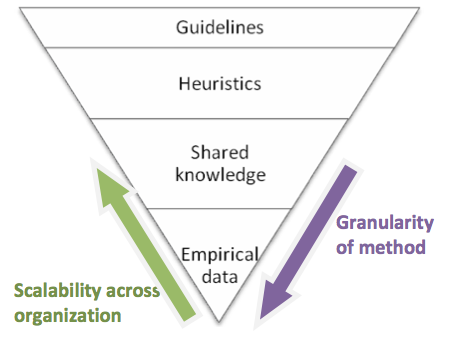
\includegraphics[width=0.5\linewidth]{Figures/api-usability-granularitaet.png}
  \caption{Skalierbarkeit von API-Evaluationsverfahren \citep{SIGCHI:2009up}}
  \label{fig:api-usability-granularitaet}
\end{figure}

Meine Arbeit ist nicht die einzige, bei der der eigentlichen Forschung eine \gls{he} vorausging. Eine andere Arbeit \citep[siehe \sref{sec:grill} und ][]{Grill:2012jm} nutzt diesen Ansatz auch --- jedoch nicht, um den Untersuchungsgegenstand für die Forschung vorzubereiten, sondern um vorab zu ermitteln, worauf sich die anschließende Erforschung fokussieren sollte. Die von mir durchgeführte \gls{he} diente jedoch lediglich der Beseitigung grober Usability-Probleme und der nicht-einschränkenden Sensibilisierung für mögliche Probleme.

Die Methode \textit{Concept Maps} \citep[siehe \sref{sec:concept-maps} und][]{Tenny:2011jp} hat sich ebenfalls als geeignet für die explorative Erforschung einer API herausgestellt. Jedoch setzt sie eine sehr hohe Einbeziehung der API-Entwickler voraus, was sich angesichts des im \sref{sec:schwierigkeiten} geschilderten \textit{technischen Wegargumentierens} \citep{Sarodnick:2006vc} als nachteilig herausgestellt haben könnte.

Das \textit{Cognitive Dimensions Framework} wird in der Forschung von \cite{clarke:2006} zur API-Usability-Evaluation eingesetzt. Wie ich bereits im \sref{sec:api-cds} beschrieben habe, ist die Darstellung des Verfahrens in der Literatur mangelhaft, was sich aber leider erst beim Versuch seiner Anwendung herausgestellt hat. Auch der Versuch, eine kostengünstige Validierung meiner im nächsten Kapitel dargestellten Forschungsergebnisse durchzuführen, ist gescheitert. Dieser Validierungsversuch wird am Ende des nächsten Kapitels (siehe \sref{sec:cdf-validation-difficulties}) erläutert.

In einer Studie zur Verbesserung einer Persistenz-Bibliothek \citep[siehe \sref{sec:piccioni} und][]{Piccioni:2013uq} wurden die kognitiven Dimensionen für APIs von \cite{Anonymous:9HSMlhmF} für die Vorbereitung von Interviewfragen genutzt. Leider ist die Zustandekommen fraglich, weil es nicht nachvollziehbar dargestellt wurde (siehe \sref{sec:cdf-usage}).

Wie bereits am Anfang dieser Arbeit gezeigt (siehe \sref{sec:gtm-informatik}), wurde die \gls{gtm} nur in drei mir bekannten und lediglich mittelbar für API-Usability-Forschung relevanten Studien \citep{Simula.simula.1294,Yamashita:2013hn,Yamashita:2013un} korrekt eingesetzt. Dabei kamen ``lediglich'' die Phasen \textit{offenes Kodieren} und \textit{axiales Kodieren} zum Einsatz. In der unmittelbar relevanten API-Usability-Forschung setzten \cite{Tenny:2011jp,deSouza:2004fd,sunshine2014searching} die \gls{gtm} nur geringfügig und mangelhaft bzw. kaum nachvollziehbar ein.


\subsection{Analyse mit Hilfe der Methode der Grounded Theory}
\label{sec:gtm-application}

Wie bereits am Anfang dieses Kapitels (siehe \sref{sec:verlauf}) beschrieben, wich meine Forschung stark von der ursprünglichen Planung ab. Die ohnehin spezielle Art der Datenerhebung und der erhobenen Daten selbst, machte die Entwicklung eines dafür geeigneten qualitativen und \gls{gtm}-unterstützenden Datenanalysewerkzeugs notwendig. Die Datenanalyse und die daraus gewonnen Erkenntnisse standen in ständiger Wechselwirkung mit den Datenerhebungen und der Werkzeugentwicklung. Beispielsweise stellte ich bei der Datenanalyse fest, dass ich nicht sehen konnte, welche Begriffe die SeqAn-Anwender in das Suchfeld der Onlinedokumentation eingegeben hatten, woraufhin ich die Datenerhebung anpassen musste (Details siehe \sref{sec:datenerhebung-probleme}). Wiederum haben die ständigen Verbesserungen von Datenerhebung und Analysewerkzeug Zeit gekostet. Der so entstandene Zeitdruck wirkte sich auf die Analysetiefe, die Auswahl der zu analysierenden Daten und schließlich auch auf die in \hyperref[sec:Ergebnisse]{Kapitel 4 vorgestellten Ergebnisse} aus.

\subsubsection{Analyse der Programmierfortschritte-Daten}

Für den ersten Analyseversuch verwendete ich den \acrfull{apiua} in Verbindung mit den während der Workshops'11 erhobenen Programmierfortschritte-Daten. Die Ergebnisse dieses Versuchs sind in \fref{fig:research-ohne-sensibilisierung} dargestellt. Als damaliger \gls{gtm}- und \acrshort{api}-Usability-Evalations-Anfänger musste ich nach insgesamt etwa drei Monaten feststellen, dass mich meine Forschung nur wenig voran gebracht hatte. Wie die Abbildung zeigt, habe ich die Programmierfortschritte unter verschiedenen Gesichtspunkten --- beispielsweise \code{apiua://code/-9223372036854775741} und \code{apiua://code/-9223372036854775734} --- analysiert.

%\newgeometry{inner=2cm,outer=1.5cm,top=1.5cm,bottom=1.5cm}
%\thispagestyle{empty}
%\begin{landscape}
\begin{figure}
  \centering
    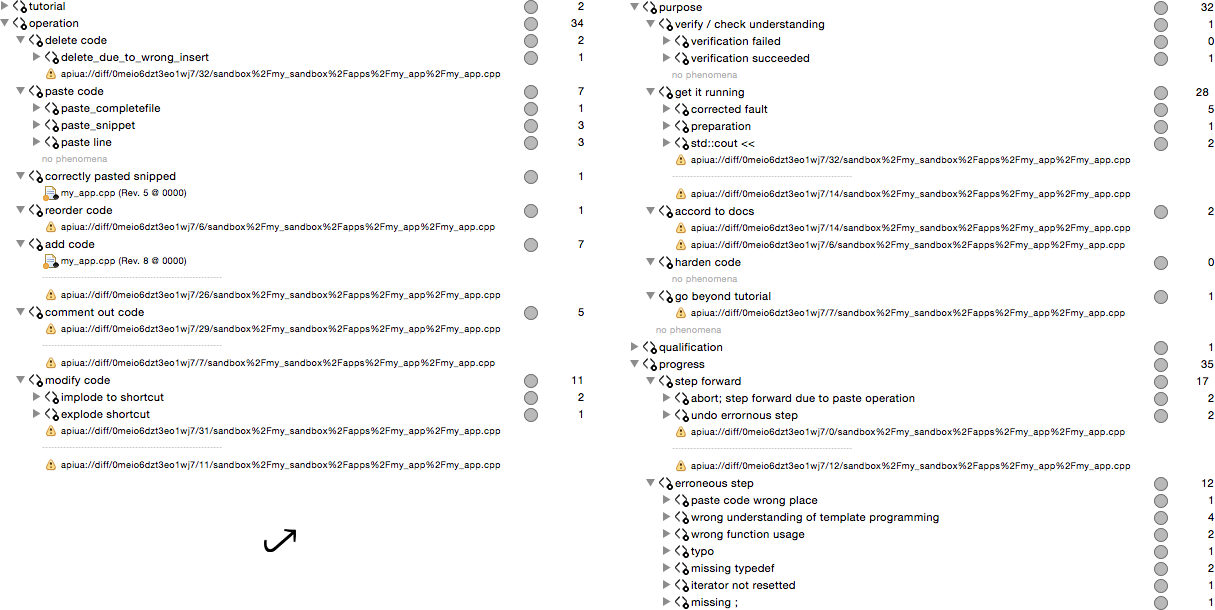
\includegraphics[width=1.0\linewidth]{Figures/research/ohne-sensibilisierung.png}
  \caption[Ergebnisse des ersten Analyseversuchs]{Ergebnisse der ersten Analyseversuchs: Die Abbildung zeigt die hierarchische Kodestruktur die bei dem ersten Versuch einer Analyse entstand. Aus technischen Gründen ist der Baum in zwei Spalten aufgetrennt. Innerhalb einer Spalte gibt es drei Spalten, von denen die erste den Namen des Kodes bzw. deren Phänomene/Verankerungen darstellt. Die grauen Linien geben an, dass aus Darstellungsgründen weite Phänomene ausgeblendet sind. Die tatsächliche Anzahl von Phänomenen steht in der dritten Spalte. Die zweite Spalte gibt die Farben der Kodes. Sie ist hier grau, weil diese Kodes nicht weiter verwendet wurde.}
  \label{fig:research-ohne-sensibilisierung}
\end{figure}
%\end{landscape}
%\restoregeometry

Ganz erkenntnislos war der erste Analyseversuch jedoch nicht. So deuteten die Kodes \code{apiua://code/-9223372036854775739} und \code{apiua://code/-9223372036854775751} bereits auf das Konzept der \code{apiua://code/-9223372036854774904} hin.% (Dem aufmerksamen Leser wird auffallen, dass die beiden Kodes damals noch nicht zusammengefasst wurden.)

Während der Analyse vollzog ich typischerweise die folgenden Schritte, die in \fref{fig:research-workflow-diff} veranschaulicht werden. Die folgenden Schritte beziehen sich auf den Kode \code{apiua://code/-9223372036854775739}:
\begin{enumerate}
  \item Zunächst habe ich einen Proband ausgewählt, dessen Programmierfortschritte ich analysieren wollte. Der entsprechende Anzeigebereich führt alle Probanden an Hand ihrer ID und ihrer Browser-Fingerprints (Details siehe \sref{sec:id}) auf. In diesem Beispiel wurde Proband \textit{0meio6dz3eo1wj7} geöffnet.
  \item Die Programmierfortschritte des Probanden können auf zweierlei Weise erkundet werden.
  \\(2a) zeigt sämtliche Aktionen des Probanden auf einer Zeitleiste:
  \\(2b) beschränkt sich auf die Darstellung der Fortschritte beim Programmieren.
  \\In diesem Beispiel interessierte mich die Datei \texttt{my\_app.cpp} der \textit{Revision 5}, die den fünften Kompilierversuch symbolisiert.
  \item Die Diff-Ansicht stellt die vorangegangene und aktuelle Version der Datei \texttt{my\_app.cpp} gegenüber. Offenbar wurden sehr viele Änderungen vorgenommen. Eine derartige, fehlerfrei wirkende Operation ist für einen SeqAn-Anfänger ungewöhnlich. Dafür musste es also eine Erklärung geben.
  \item Der Bereich (4a) stellt listenartig alle Ereignisse auf der Online-Dokumentation dar. Der Bereich (4b) stellt dieselben Informationen in der untersten Zeile der Zeitleiste dar. Der bläuliche Einfärbung auf der Zeitleiste markiert dabei den Zeitraum des Workshops. Die neongrünliche Einfärbung hebt sämtliche Ereignisse hervor, die in die Zeitspanne der Arbeiten an der fünften Revision der Datei \texttt{my\_app.cpp} fallen.
  \\Bleibt der Forscher mit der Maus über einem Ereignis stehen, werden detaillierte Informationen in (5) dargestellt.
  \item Der Detaildialog ist ein nicht-modales Fenster, wie man es aus der Eclipse-Entwicklungsumgebung, beispielsweise bei der Codevervollständigung kennt. In diesem Fall zeigt das Fenster an, was genau der Proband in diesem Moment auf der Online-Dokumentation gesehen hat. Der blasse Pfeil im Hintergrund des Screenshots bedeutet, dass der Anwender herunter gescrollt ist, um den dargestellten Bereich zu sehen. Der Screenshot zeigt ein SeqAn-Online-Tutorial. Durch den Vergleich des Tutorial-Inhalts mit dem, was der Anwender programmiert hat, wird deutlich, dass er zwei Code-Fragmente aus dem Tutorial kopiert und in seiner C{}\verb$++$-Datei eingefügt hat.
  \item Die beiden Fragmente habe ich mit dem Kode \code{apiua://code/-9223372036854775739} kodiert. Da die Kodeansicht alle existierenden Kodes darstellt, bietet es sich an dieser Stelle an, die Kodierung mit den bereits kodierte Phänomenen im Sinne des \textit{ständiges Vergleichens} gegenüberzustellen, um zu klären, ob es sich wirklich noch um die Semantik des Kodes handelt.
  \item Erkenntnisse können in der Memoansicht festgehalten werden. In diesem Fall war das Memo bereits in Kode \code[apiua://code/-9223372036854775750]{paste\_snippet} festgehalten, der mit \code{apiua://code/-9223372036854775739} zusammengefasst werden sollte.
  \item Die Kodierung der fünften Revision der Datei \texttt{my\_app.cpp} ist abgeschlossen. Die Programmierfortschritte-Ansicht kann nun verwendet werden, um die sechste Revision zu kodieren.
\end{enumerate}

\newgeometry{inner=2cm,outer=1.5cm,top=1.5cm,bottom=1.5cm}
\thispagestyle{empty}
\begin{landscape}
\begin{figure}
  \centering
    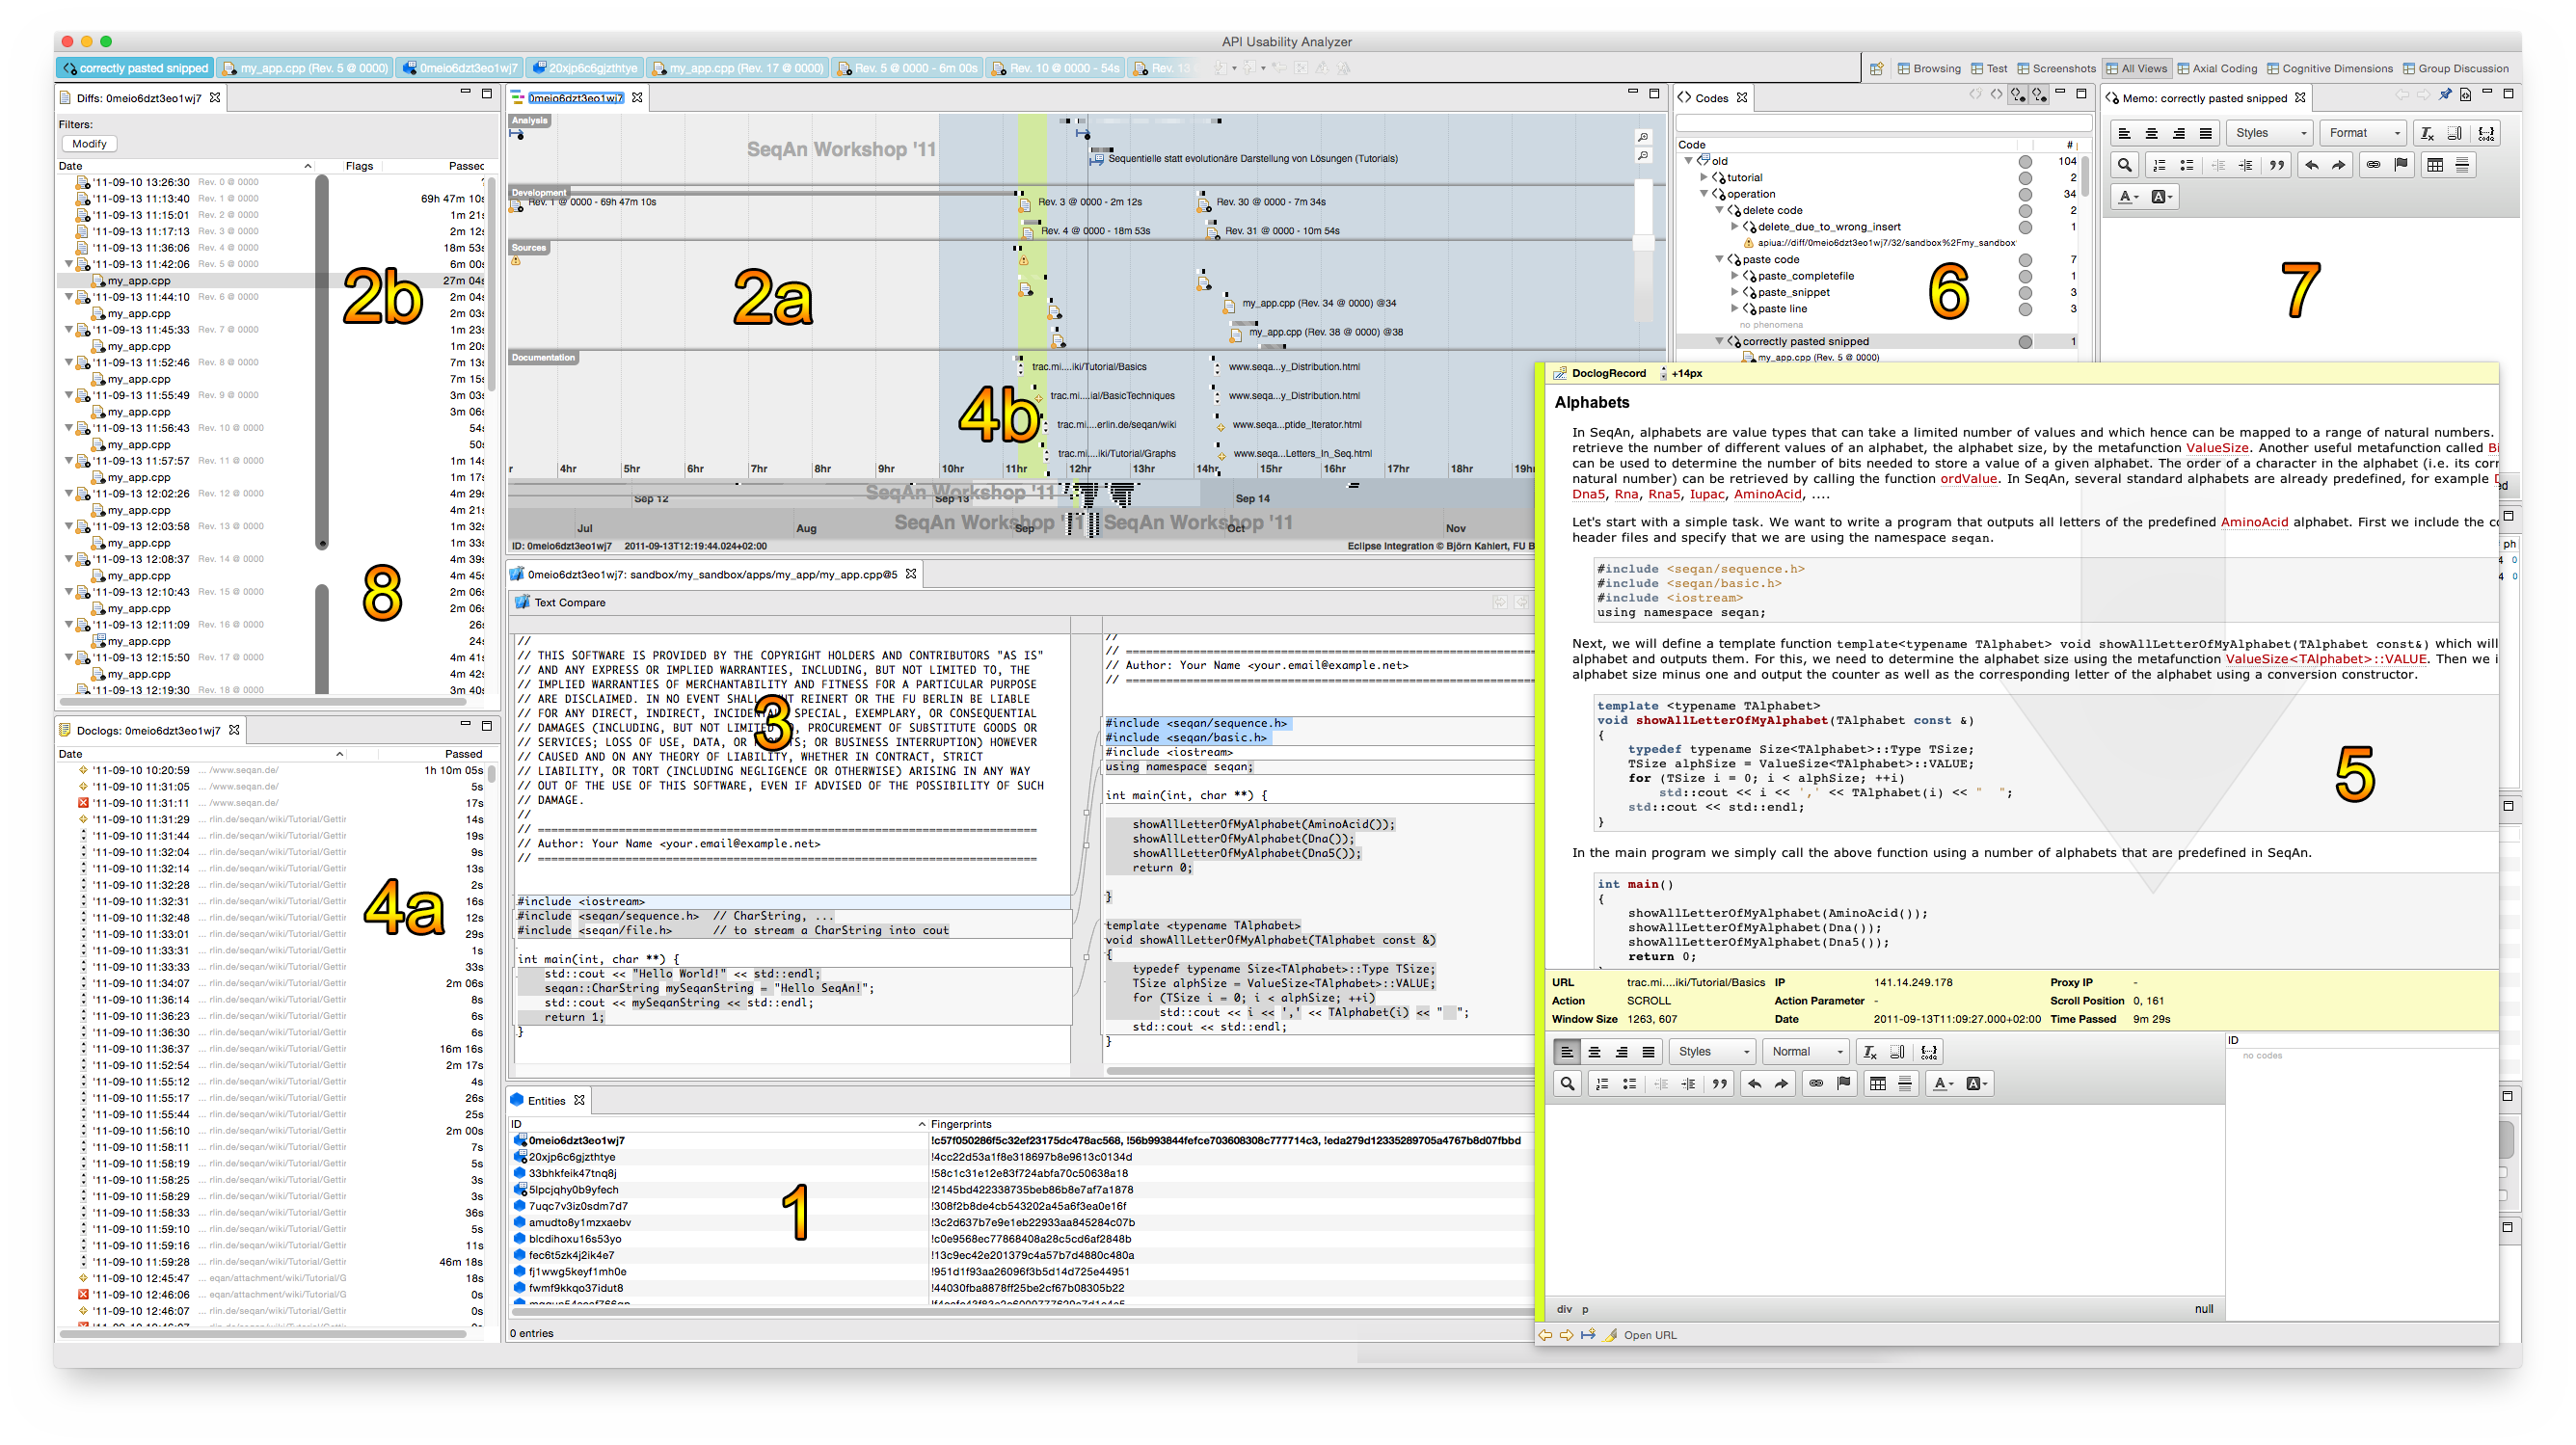
\includegraphics[width=1.0\linewidth]{Figures/research/workflow-diff.png}
  \caption[Analyse von Programmierfortschritte-Daten mit Hilfe von APIUA]{Analyse von Programmierfortschritte-Daten mit Hilfe von APIUA: (1) Auswahl des Probanden, dessen Programmierfortschritte analysiert werden sollen. (2a) zeigt die Programmierfortschritte entlang einer Zeitleiste. (2b) beschränkt sich auf eine Listendarstellung. (3) stellt die vorangegangene und aktuelle Version der selektierten Datei gegenüber. (4a) stellt listenartig alle Ereignisse auf der Online-Dokumentation dar. (4b) Dasselbe macht unterste Zeile der Zeitleiste. (5) stellt detaillierte Informationen zu einem Datenpunkt dar. (6) zeigt die existierenden Kodes. In (7) werden Erkenntnisse zum aktuell selektierten Element festgehalten. Wurde die betrachtete Datei kodiert, kann der Forscher in (8) fortfahren.}
  \label{fig:research-workflow-diff}
\end{figure}
\end{landscape}
\restoregeometry


Auch wenn man auf diese Weise sehr gründliche Analysen durchführen kann, erfordert es viel Übung, ein gewisses Abstraktionsniveau zu erreichen, welches dem selbst gesteckten Ziel genügt. In meinem Fall war dies die Erforschung und insbesondere die Verbesserung der API-Usability von SeqAn.

Um meine Sensibilität zu erhöhen und eine effizientere, gezieltere Analyse der objektiven Programmierfortschritte-Daten zu erreichen, habe ich mich entschlossen, zunächst mit der Analysen der subjektiven Datenquellen \textit{Cognitive-Dimensions-Fragebogen} und \textit{Gruppendiskussion} fortzufahren. Immerhin konnten die Forscher der API-Usability-Studie von \cite{Grill:2012jm} 55\% der entdeckten Usability-Probleme in der direkten Interaktion mit Benutzern (insb. Interviews) finden.



\subsubsection{Analyse der Cognitive-Dimensions-Fragebögen}

Die im \sref{sec:cdf-usage} vorgestellten Cognitive-Dimensions-Fragebögen kamen am Ende des Workshops'13 zum Einsatz. \fref{fig:research-workflow-cdf} zeigt, wie die entsprechende Analyseansicht in \gls{apiua} aussieht. Der Kodierprozess ist dem im vorangegangenen Abschnitt ähnlich genug, um ihn an dieser Stelle kein zweites Mal zu erläutern.

\begin{figure}
  \centering
    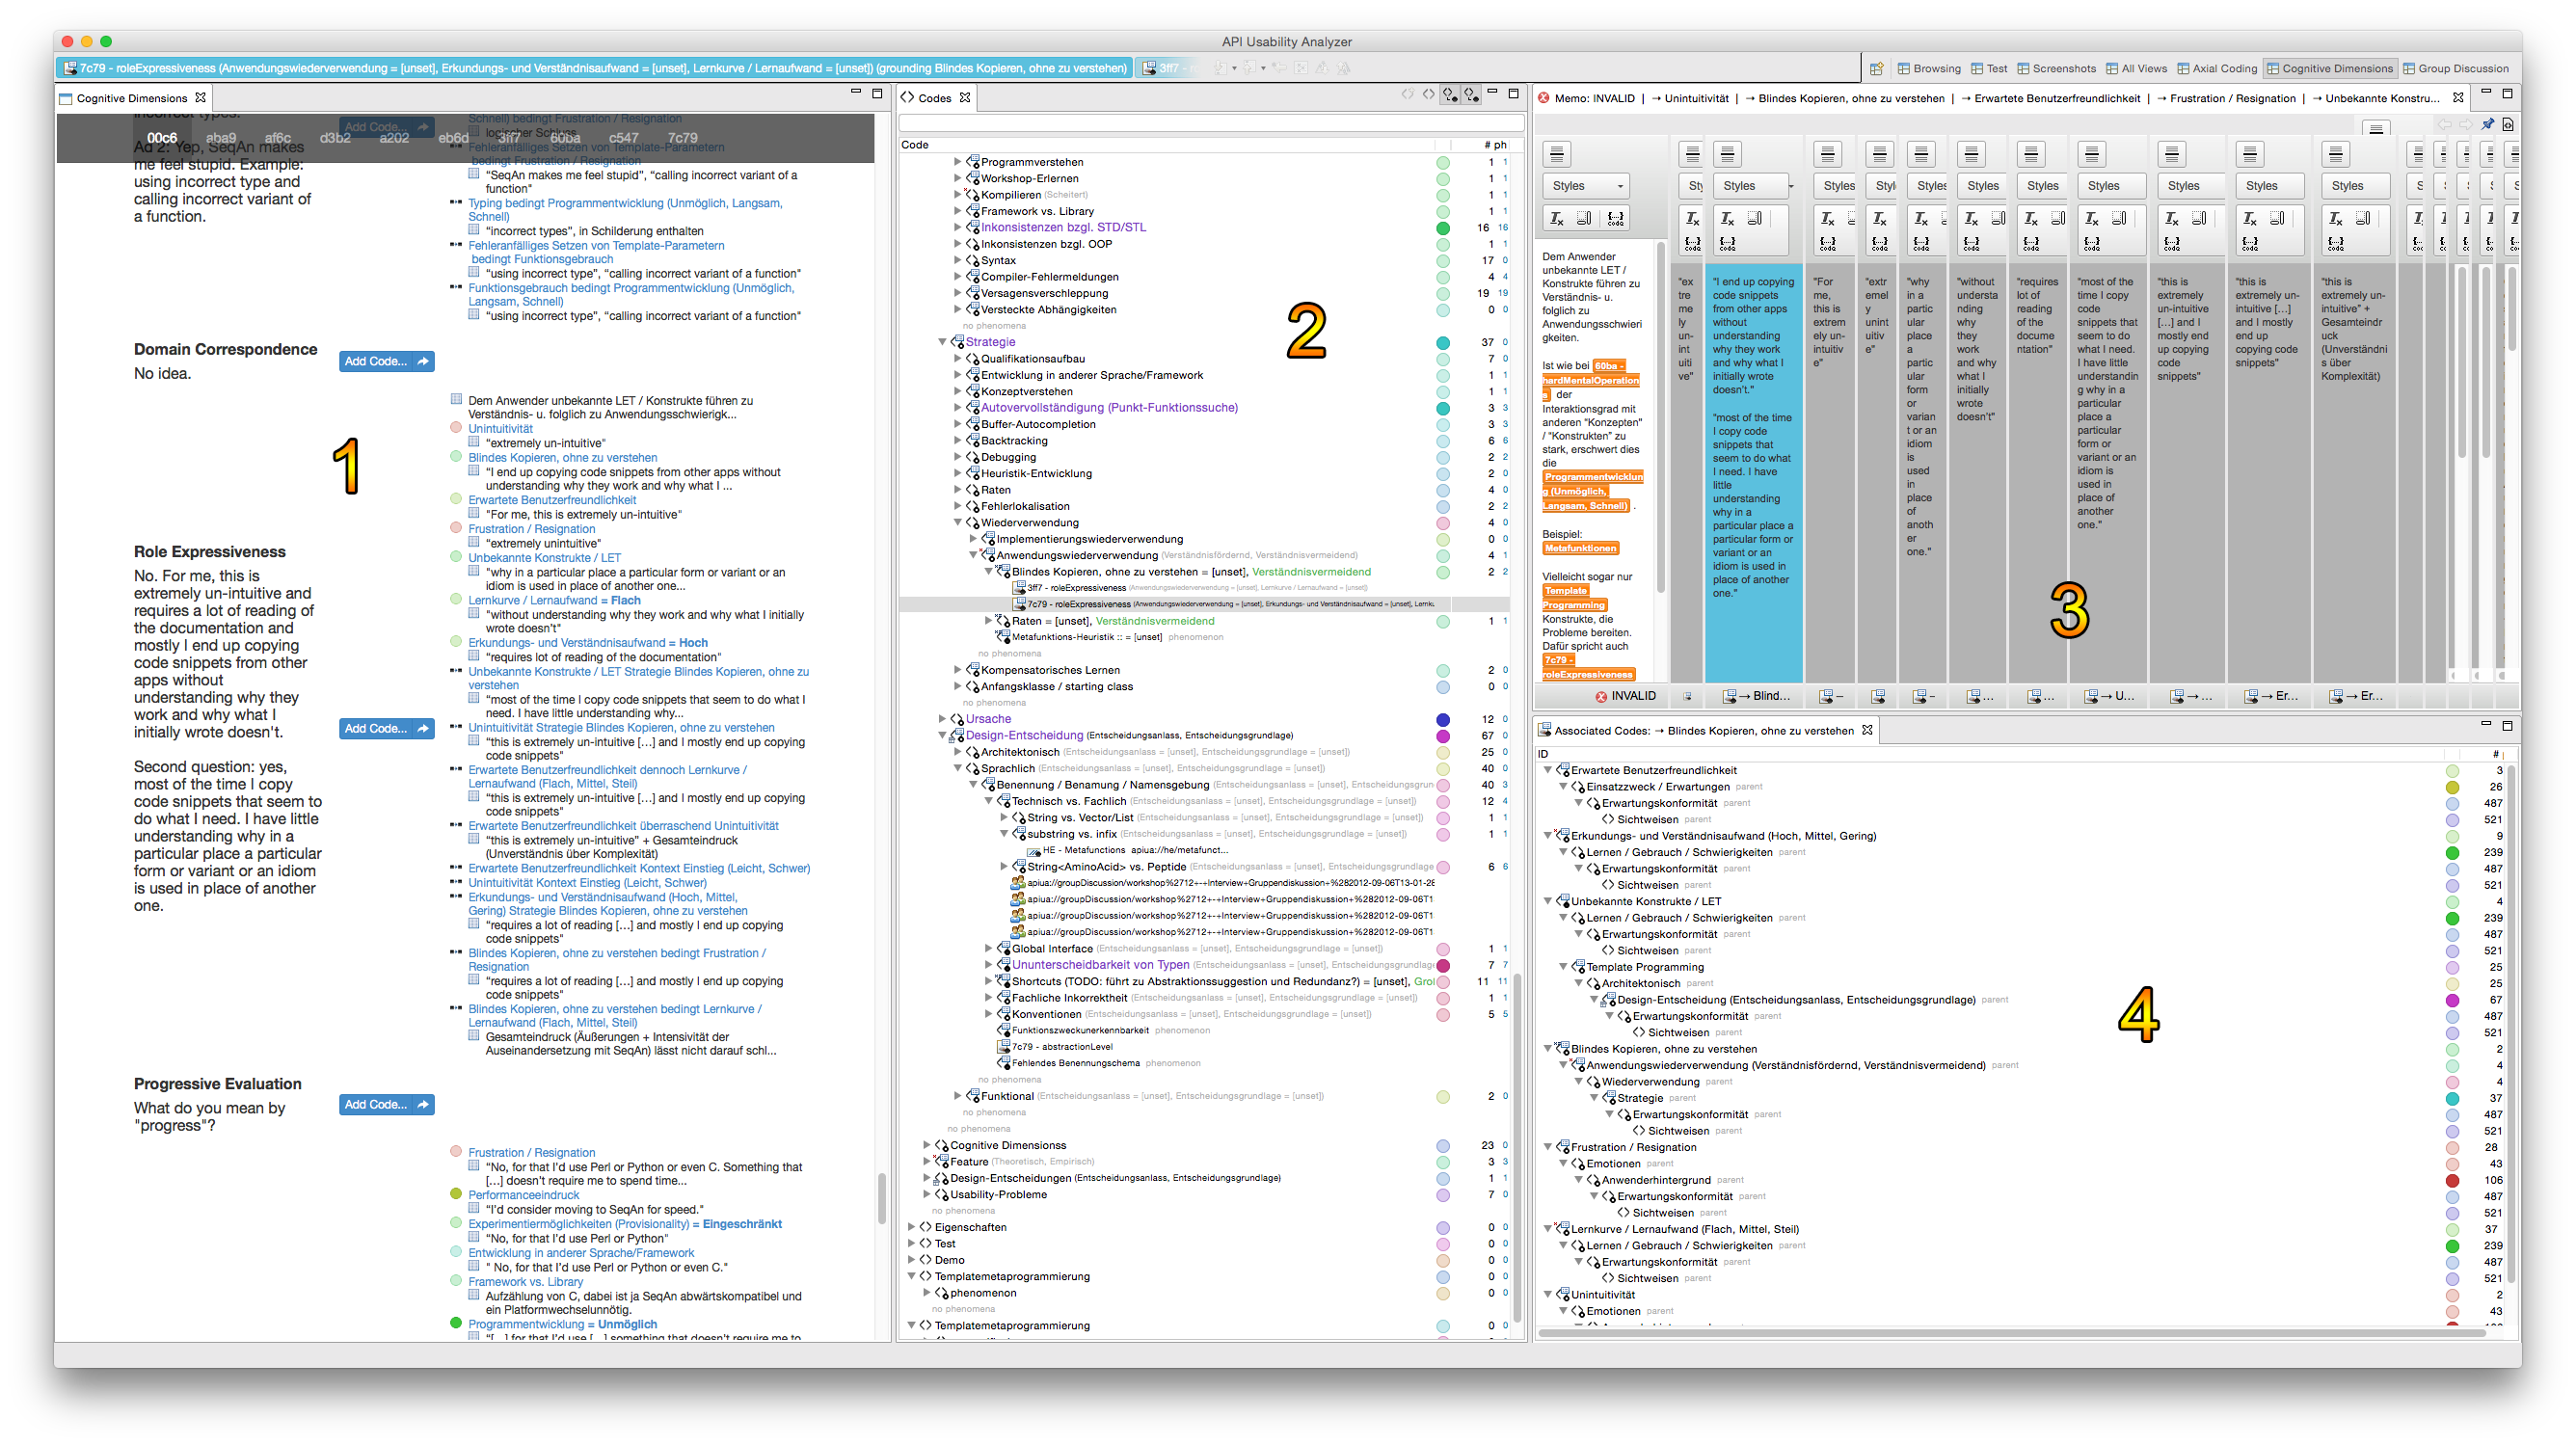
\includegraphics[width=1.0\linewidth]{Figures/research/workflow-cdf.png}
  \caption[Analyse der Cognitive-Dimensions-Fragebögen mit Hilfe von APIUA]{Analyse der Cognitive-Dimensions-Fragebögen mit Hilfe von APIUA: (1) Dieser Bereich stellt alle Antworten der Fragebögen dar. (2) zeigt alle gefundenen Kodes. Neben einem Kode ist dessen Dimensionalisierung dargestellt. Unterhalb eines Kodes sind die Fundstellen/Phänomene aufgelistet. (3) stellt das Memo des aktuell selektierten Elements (blau hervorgehoben), das Memo des zur Selektion gehörenden Kodes (weiß) und die Memos der anderen dem Phänomen zugewiesenen Kodes (grau) dar. (4) listet die zugewiesenen Kodes und deren Elternkode-Hierarchie auf.}
  \label{fig:research-workflow-cdf}
\end{figure}

Die Analyse der Fragebögen war weitaus ergiebiger, auch wenn sie mehrere Monate umfasste. In keiner Datenquelle fand ich so viele Informationen zur Kategorie \code{apiua://code/-9223372036854775237} (u.a. \code{apiua://code/-9223372036854775280} und \code{apiua://code/-9223372036854775279}, siehe \pageref{sec:gt-funktionsbezogene-probleme}) wie in dieser.

An das Beispiel der \code{apiua://code/-9223372036854774904} anknüpfend, konnte ich bei der Analyse der Fragebögen den Kode \code{apiua://code/-9223372036854775508} entdecken. Ein solcher Bezeichner klingt zunächst nach einer mutigen Behauptung, die mit den Programmierfortschritte-Daten --- ohne entsprechende Übung --- nicht einfach zu belegen wäre. In dieser subjektiven Datenquelle fiel das deutlich leichter. So hat beispielsweise ein Proband zu der Frage zur CD \textit{Rolenerkennbarkeit} gesagt: ``[Writing code] is extremely un-intuitive [\dots] and mostly I end up copying code snippets from other apps without understanding why they work''\citepurl{apiua://survey/cd/2013-09-19T11:51:16.616+02:00/domainCorrespondence}.

Manche Fragen wurden von Teilnehmer nicht so verstanden, wie ich das beabsichtigte (Details siehe \sref{sec:cdf-usage}
). Das stellt zwar Forscher vor ein Problem, wenn sie den Fragebogen im Sinne des Cognitive Dimensions Frameworks (siehe Abschnitte \ref{sec:cdf} und \ref{sec:api-cds}) auswerten wollen. Für die \gls{gtm}-Analyse ist dies jedoch unproblematisch, geben die Befragten ja dennoch relevante und wertvolle Informationen.

Bis eben habe ich mich lediglich auf das \textit{offene Kodieren} beschränkt. Für das \textit{axiale Kodieren} waren die Fragebögen weniger geeignet, denn ihnen fehlt weitgehend der Prozesscharakter, der in den Programmierfortschritte-Daten inherent vorhanden ist. Bei den Fragebögen haben die meisten Antworten einen resümierenden, momentbezogenen Charakter, was axiales Kodieren im Sinne des \textit{paradigmatischen Modells} (siehe \sref{sec:gtm}) erschwert. Viele meiner erarbeiteten \textit{\glslink{ac}{axialen Kodierungen}} geben daher auch eher ein Résumé bzw. einen Kausalitätsgraphen wieder. \fref{fig:research-cdf-eb6d} zeigt ein entsprechendes einfaches Beispiel.

\begin{figure}
\begin{minipage}{\textwidth}
  \centering
    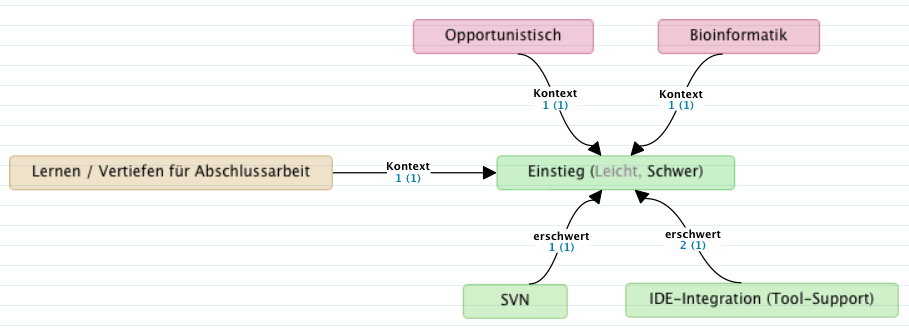
\includegraphics[width=0.75\linewidth]{Figures/research/cdf-eb6d.png}
  \caption[Kausale axiale Kodierung]{Einfache kausale axiale Kodierung\citepurl{apiua://axialcodingmodel/KfDWvbBWybMDxf5O} eines Teilnehmers\citepurl{apiua://survey/cd/2013-09-18T17:46:05.890+02:00}}
  \label{fig:research-cdf-eb6d}
\end{minipage}
\end{figure}

In \fref{fig:research-workflow-cdf} (Bereich 2) kann man bereits erahnen, wie erkenntnisreich die zehn analysierten Fragebögen waren. Ich entschloss mich also, mit der Analyse der zweiten subjektiven Datenquelle \textit{Gruppendiskussion} fortzufahren.



\subsubsection{Analyse der Gruppendiskussion}

In der im \sref{sec:gruppendiskussion} vorgestellten und beim Workshop'12 durchgeführten Gruppendiskussion verwendete ich das Programmierparadigma \textit{Templatemetaprogrammierung} als Hauptreiz. Weitere Reizargumente habe ich hauptsächlich auf der Grundlage von zuvor ausgegebenen Feedback-Zetteln erarbeitet (Details siehe \sref{sec:gruppendiskussion}).

Neben den zu beobachtenden Wiederverwendungsstrategien gaben die Cognitive-Dimensions-Fragebögen umfangreich Aufschluss über unterschiedliche Facetten zur, in SeqAn verwendeten \code{apiua://code/-9223372036854775515}. Ein zuvor unentdeckter Aspekt sind \code[apiua://code/-9223372036854775633]{Inkonsistenzen bzgl. STL} (\textit{STL} steht für die \textit{C}\verb$++$ \textit{Standard Template Library}\footnote{Diese Bezeichnung ist eigentlich nicht ganz korrekt, denn die Standard Template Library (ohne~C++) ist eine von Alexander Stepanov entwickelte Softwarebibliothek für generische Programmierung \citep{TheStandardTemplat:1994vd}, die 1998 in die C++ Standard Library aufgenommen wurde (ISO/IEC 14882:1998).}), die einen Schwerpunkt der Diskussion selbst und meiner mehrmonatigen Analyse darstellte. Die gewonnenen Erkenntnisse sind ein zentraler Punkt meiner im nächsten Kapitel vorgestellten \gls{gt}, weshalb ich an dieser Stelle nicht weiter darauf eingehe.

\fref{fig:research-workflow-gd} zeigt die \gls{apiua}-Perspektive zur Analyse von Gruppendiskussion und veranschaulicht meine Arbeitsweise mit dem \gls{apiua}-Werkzeug.

\begin{figure}
\begin{minipage}{\textwidth}
  \centering
    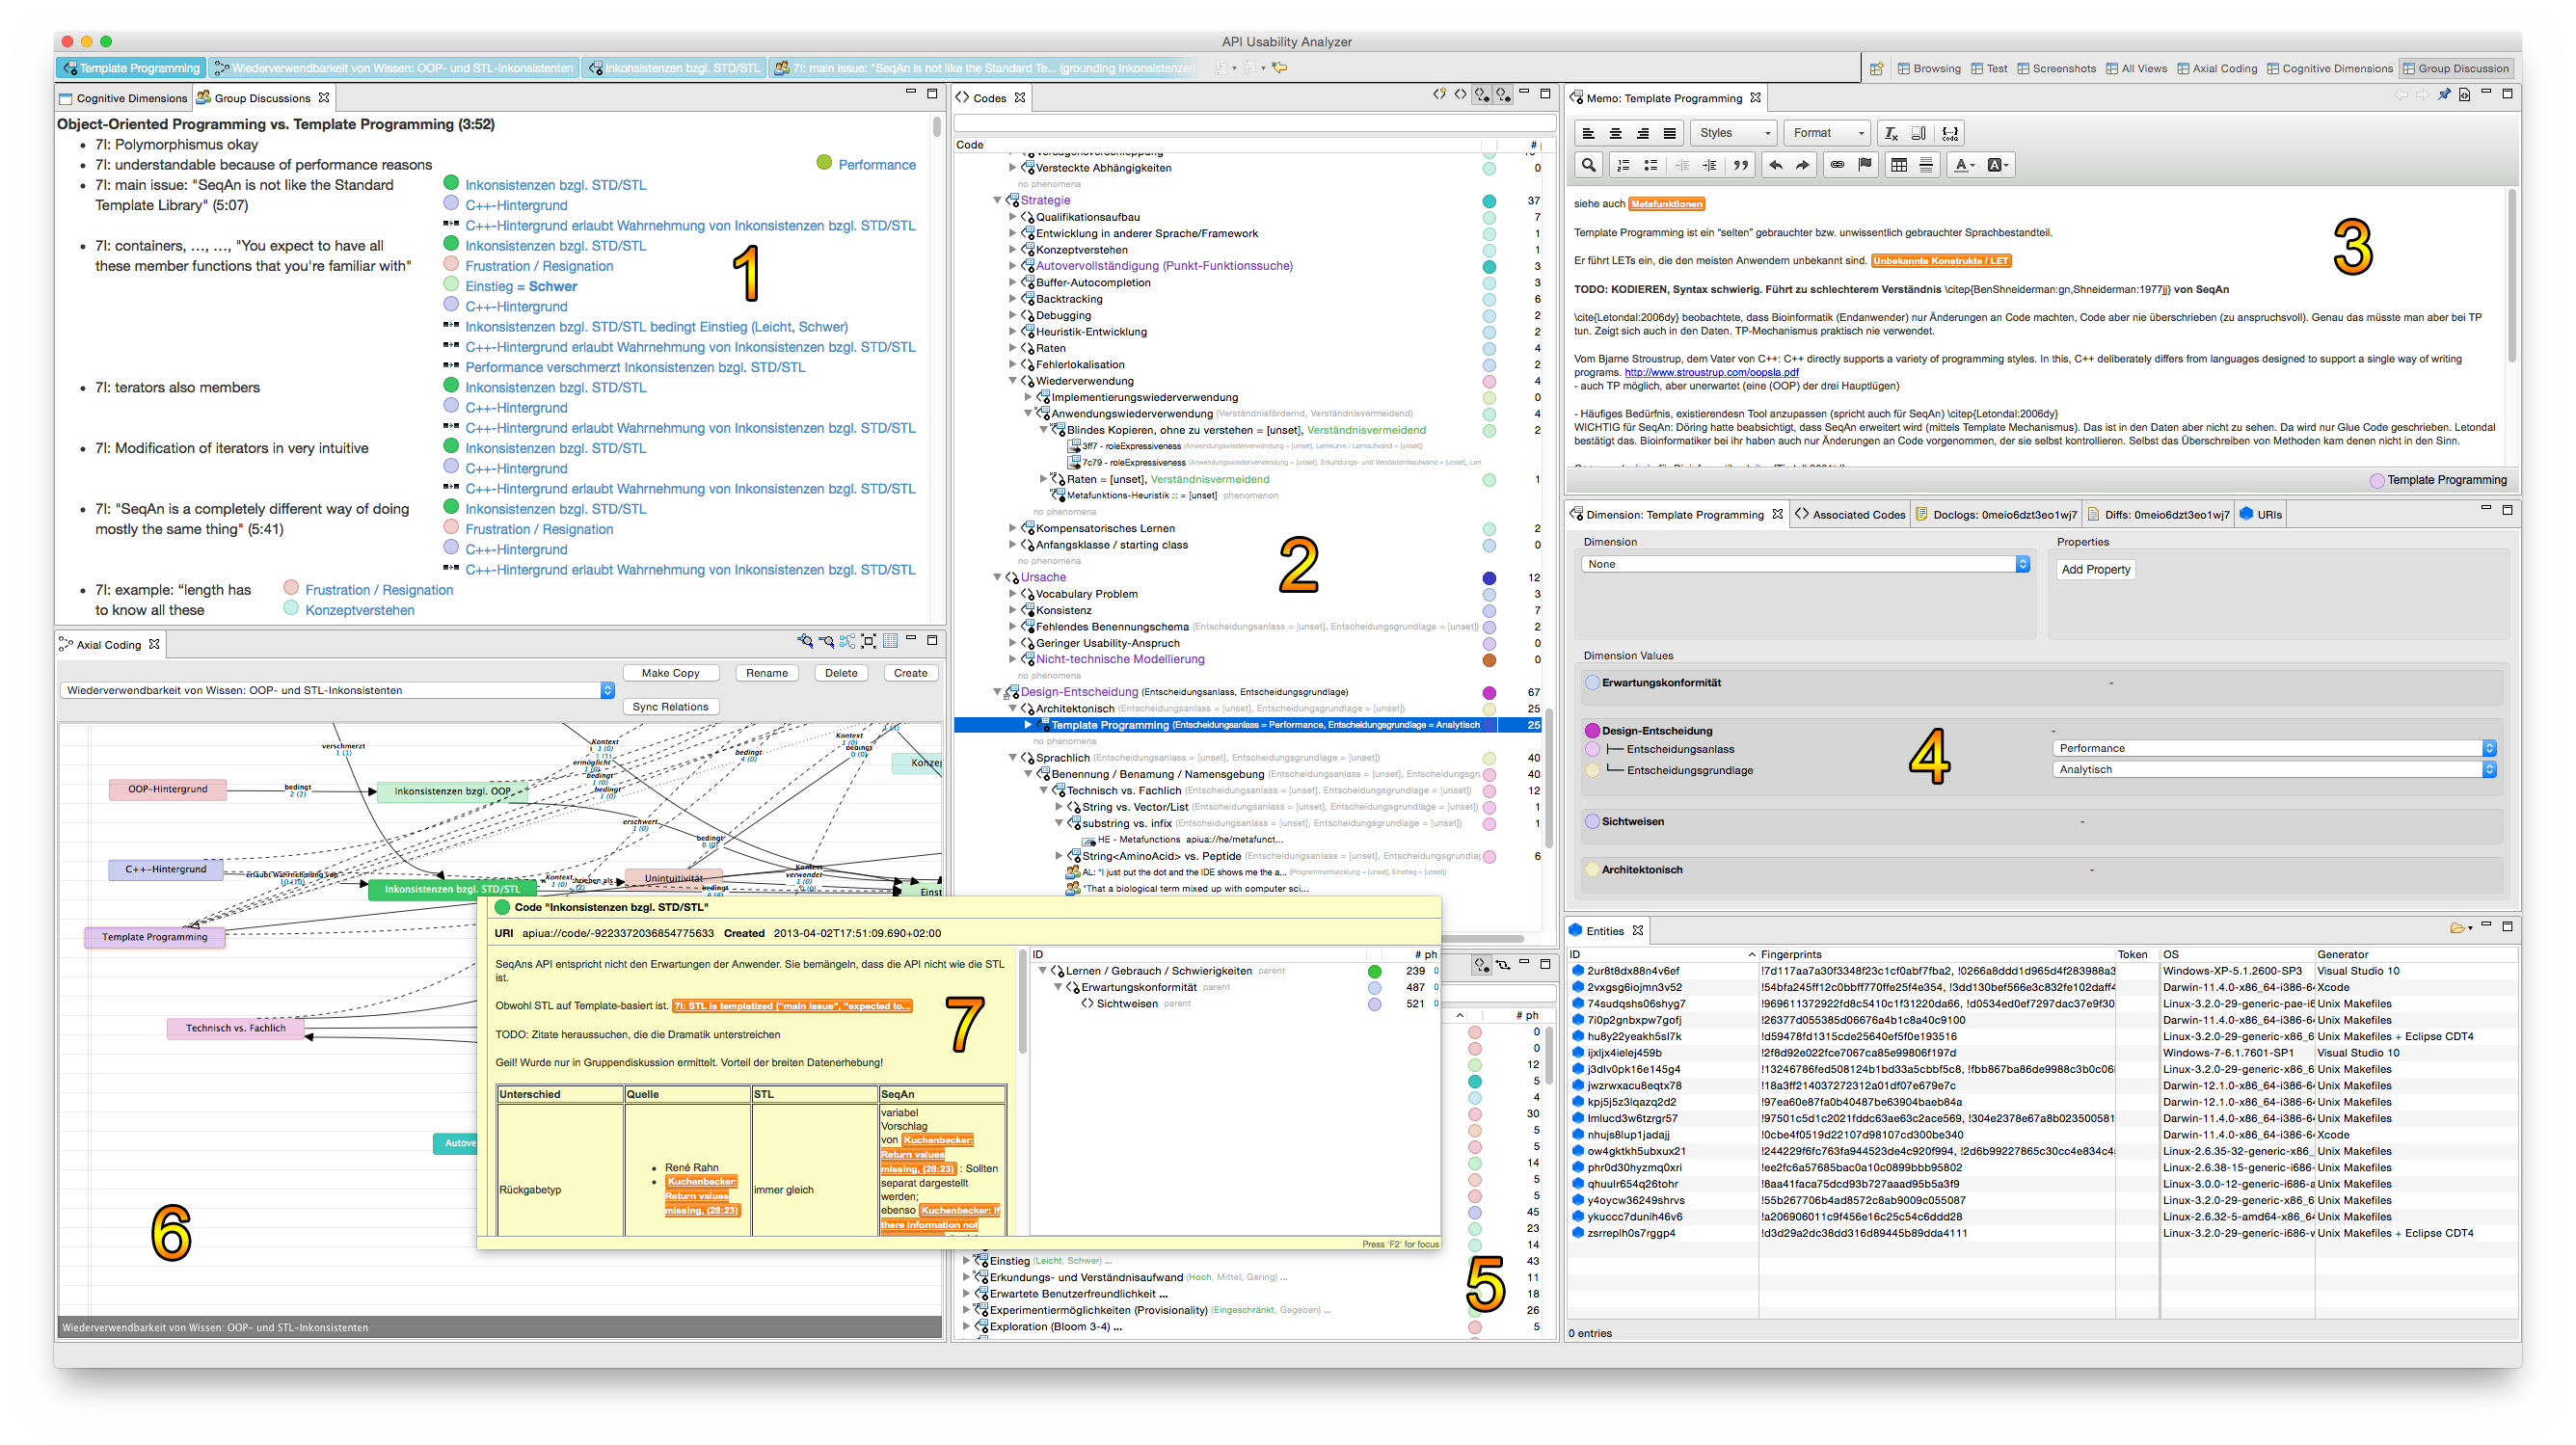
\includegraphics[width=1.0\linewidth]{Figures/research/workflow-gd.png}
  \caption[Analyse der Gruppendiskussion mit Hilfe von APIUA]{Analyse der Gruppendiskussion mit Hilfe von APIUA: (1) zeigt das informelle Transkript der Gruppendiskussion. (2) zeigt die gefundenen Konzepte. (3) zeigt das Memo zur \code{apiua://code/-9223372036854775515}. (4) zeigt die von \code{apiua://code/-9223372036854775281} gererbten Eigenschaften von \code{apiua://code/-9223372036854775515}: \code{apiua://code/-9223372036854774942} und \code{apiua://code/-9223372036854774839}. (5) zeigt die gefundenen Relationen, wie z.B. \rel[bedingt\citepurl{apiua://relation/ir9b27ic23kv7jhi617vnf8u5kvclc59}]{\code[apiua://code/-9223372036854775633]{Inkonsistenzen bzgl. STL}}{\code[apiua://code/-9223372036854775262]{Einstieg (schwer)}}. (6) zeigt ein relevantes \gls{acm}\citepurl{apiua://axialcodingmodel/QpPaMj4mceVnuSYI}. (7) stellt in einem schwebenden Dialog das Memo zum gerade selektierten Kode \code[apiua://code/-9223372036854775633]{Inkonsistenzen bzgl. STL} dar.}
  \label{fig:research-workflow-gd}
\end{minipage}
\end{figure}



\subsubsection{Erneute Analyse der Programmierfortschritte-Daten}

Mit der neu gewonnen Sensibilisierung für SeqAn-Usability-Probleme, wollte ich meine erhobenen Programmierfortschritte-Daten ein weiteres Mal analysieren. Wegen des enormen Zeitdrucks (siehe \sref{sec:schwierigkeiten}) habe ich nur eine Handvoll bereits beobachteter Usability-Probleme, wie die \code{apiua://code/-9223372036854774846}, trianguliert.

Auf die Analyse der 1.200 Revisionen umfassenden Langzeitbeobachtung musste ich leider ganz verzichten.

Wie die im nächsten Kapitel vorgestellte \gls{gt} zeigen wird, gab es allerdings auch keine zwingende Notwendigkeit einer zweiten Analyse der Programmierfortschritte. Dies soll nicht bedeuten, dass diese Analyse nicht wertvoll und erkenntnisreich gewesen wäre. Allerdings musste ich mich entschließen, diesen Analyseschritt für zukünftige Forschungsvorhaben aufzusparen.



\subsubsection{Selektives Kodieren}

Im Verlauf meiner Forschung analysierte ich fortwährend meine automatisch generierten und händisch angepassten \glslink{acm}{axialen Kodiermodelle}, um Erklärungs- und Kausalitätslücken an Hand meiner erfassten Daten zu füllen. Dabei platzte geradezu der Knoten, als ich versuchte, das Konzept \code{apiua://code/-9223372036854775633} axial zu kodieren (siehe \fref{fig:research-gt-vorlage}). Im Nachhinein würde ich diesen Moment als \textit{abduktiven Blitz}\footnote{\cite{Strubing:2005ve} zitiert den Begründer des \textit{abduktiven Schließens} Charles Sanders Peirce wie folgt: ``Die abduktive Vermutung <suggestion> kommt uns wie ein Blitz. Sie ist ein Akt der \textit{Einsicht}, obwohl extrem fehlbarer Natur. Zwar waren die verschiedenen Elemente der Hypothese schon vorher in unserem Verstande; aber erst die Idee, das zusammenzubringen, welches zusammenzubringen wir uns vorher nicht hätten träumen lassen, läßt die neu eingegebene Vermutung vor unser Betrachtung aufblitzen''} beschreiben. \label{sec:abduktiver-blitz}

\begin{figure}
\begin{minipage}{\textwidth}
  \centering
    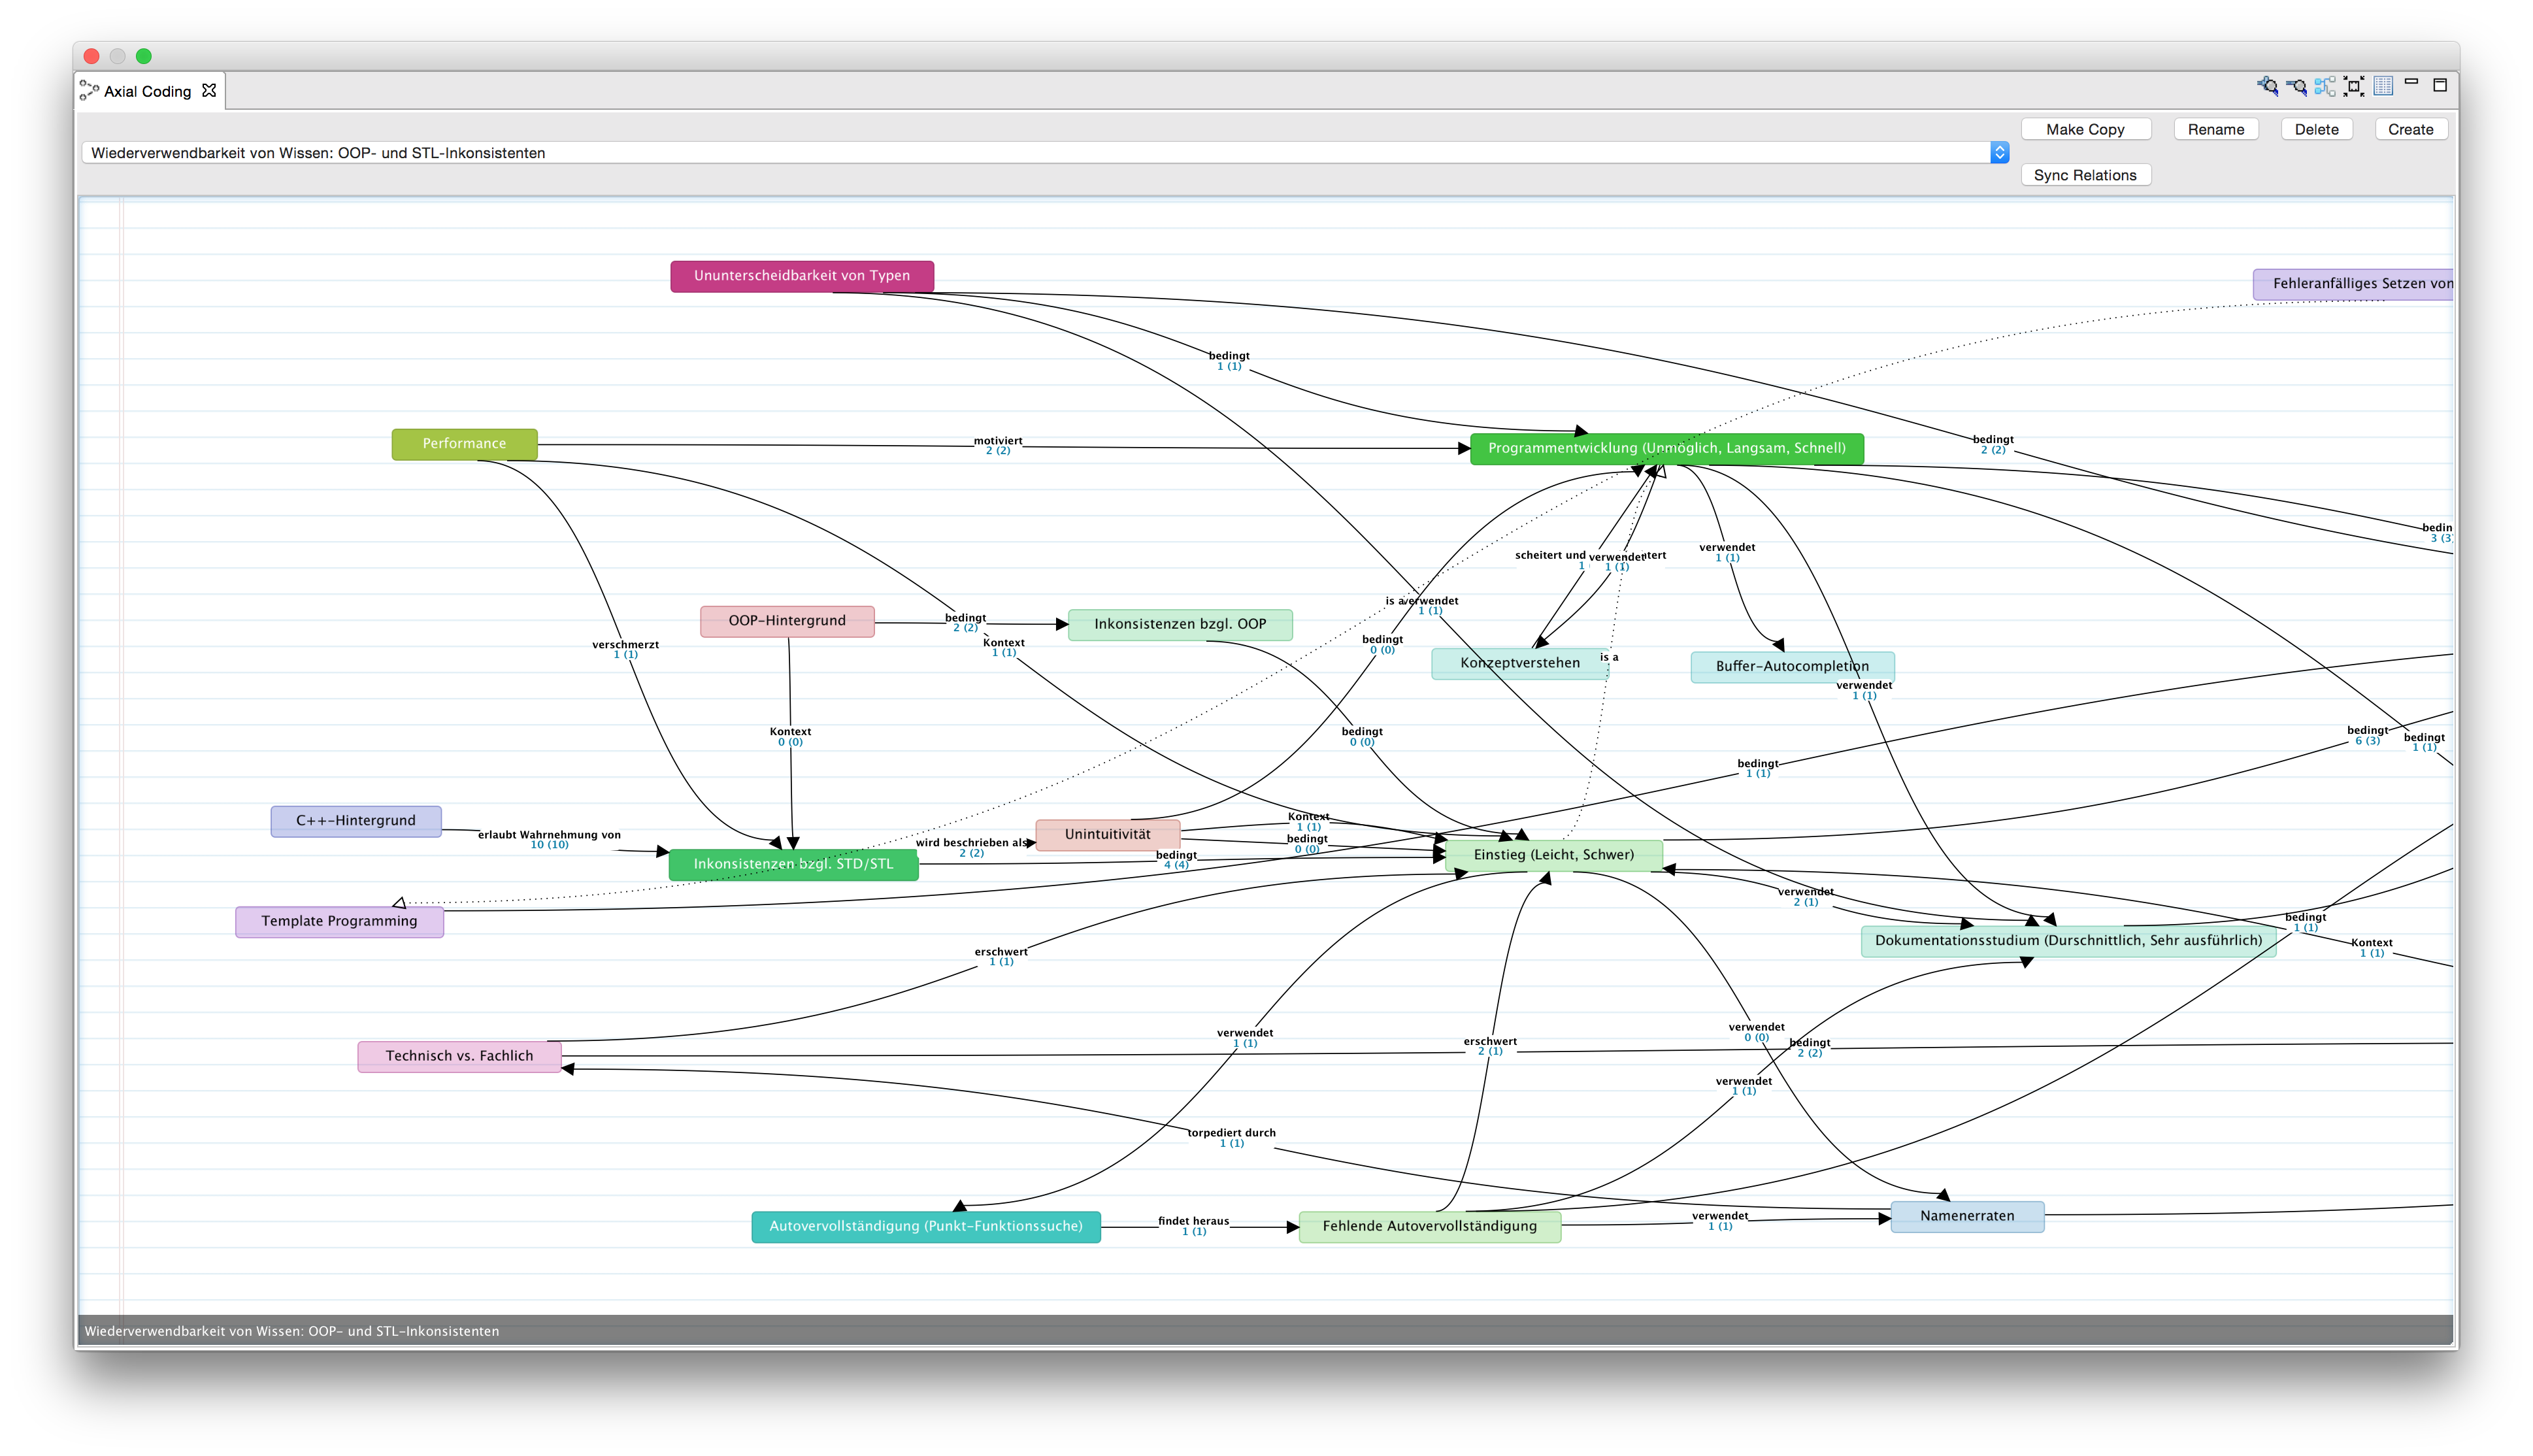
\includegraphics[width=1.0\linewidth]{Figures/acm/stl-inconcistencies-old.png}
  \caption{Axiale Kodierung des Konzepts \code{apiua://code/-9223372036854775633}}
  \label{fig:research-gt-vorlage}
\end{minipage}
\end{figure}

Ich stellte mir die Frage, worin sich \code{apiua://code/-9223372036854775633} und \code{apiua://code/-9223372036854775080} unterscheiden. Mir wurde plötzlich klar, dass die \code{apiua://code/-9223372036854775494}\footnote{Darunter verstehe ich einfach ausgedrückt, welche Paradigmen (objektorientierte Programmierung, Templatemetaprogrammierung, etc.) von einem Anwender auf Grund seiner Ausbildung oder Tätigkeit besonders präferiert und damit besonders gut beherrscht werden.} der Anwender eine elementare Rolle in der Bewertung der API-Usability spielt. In diesem Erklärungsansatz fühlte ich mich durch die Beobachtung bestätigt, dass sich der Gebrauch der Strategie \code{apiua://code/-9223372036854775145}\footnote{Darunter verstehe ich die Auflistung zur Verfügung stehender Funktionen durch die Eingabe eines Punktes nach einer Variablen innerhalb der eigenen IDE.} ebenfalls damit erklären ließ.

Abstrakt betrachtet, war allen Anwendern gemeinsam, dass sich die Usability von SeqAn signifikant aus den Vorerfahrungen und Vorkenntnissen seiner Anwender ergab, was ich als \textit{Erwartungskonformität} bezeichnet habe, und die Perspektive für  das selektive Kodieren darstellte.

Je mehr ich wichtige von weniger wichtigen Konzepten unterschied, desto deutlicher wurde, dass eine ganze Reihe von unempirischen \code{apiua://code/-9223372036854775281} ursächlich für die von mir beobachteten Usability-Probleme war.

Beim selektiven Kodieren habe ich ein ganzheitliches axiales Kodiermodell entwickelt\citepurl{apiua://axialcodingmodel/Yty2pVeMWuNS2BoX}, das durch einen sehr hohen Komplexitätsgrad gekennzeichnet war (siehe \fref{fig:research-gt1}). Um dieses in seiner Komplexität, aber dennoch sinnerhaltend zu reduzieren, entwickelte ich eine APIUA-Funktion, die es mir erlaubte, Relationen zu abstrahieren, d.h. entlang der Konzept-Hierarchien der verbundenen Konzepte nach oben zu bewegen. Ob es sich dabei um eine legitime Operation handelt, konnte ich durch die APIUA-Funktion der hypothetischen Relationen (siehe \sref{sec:Erkenntnisperspektive}) beantworten. Auf diese Weise konnte ich in dem Dickicht an gefundenen Relationen solche finden, die zusammengefasst und abstrahiert werden können.

Schienen hypothetische Relationen vollkommen unpassend, deutete dies auf Modellierungsschwächen hin. Beispielsweise waren die Folgen von \code{apiua://code/-9223372036854775514} (\code{apiua://code/-9223372036854775513} und \code{apiua://code/-9223372036854775511}) fälschlicherweise Unterkonzepte von \code{apiua://code/-9223372036854775514} selbst. Das Verschieben dieser Folgen in den anderen Teilbaum \code{apiua://code/-9223372036854775405} entsprach mehr der in den Daten manifesten Ordnung und reduzierte die Komplexität des zunehmend theoretischen Modells (siehe \fref{fig:research-workflow-selectivecoding-c}). Das Zwischenergebnis nach gut fünf Wochen aufwändigen selektiven Kodierens zeigt \fref{fig:research-gt2}\footnote{Leider kam das selektive Kodieren auf derart ungünstige Weise ins Stocken, dass ich die Diagnose und die Behebung des Problems im \aref{app:acm-editor-problem} ausführlicher beschreibe.}.

\begin{figure}
        \centering
        \begin{subfigure}{0.48\linewidth}
                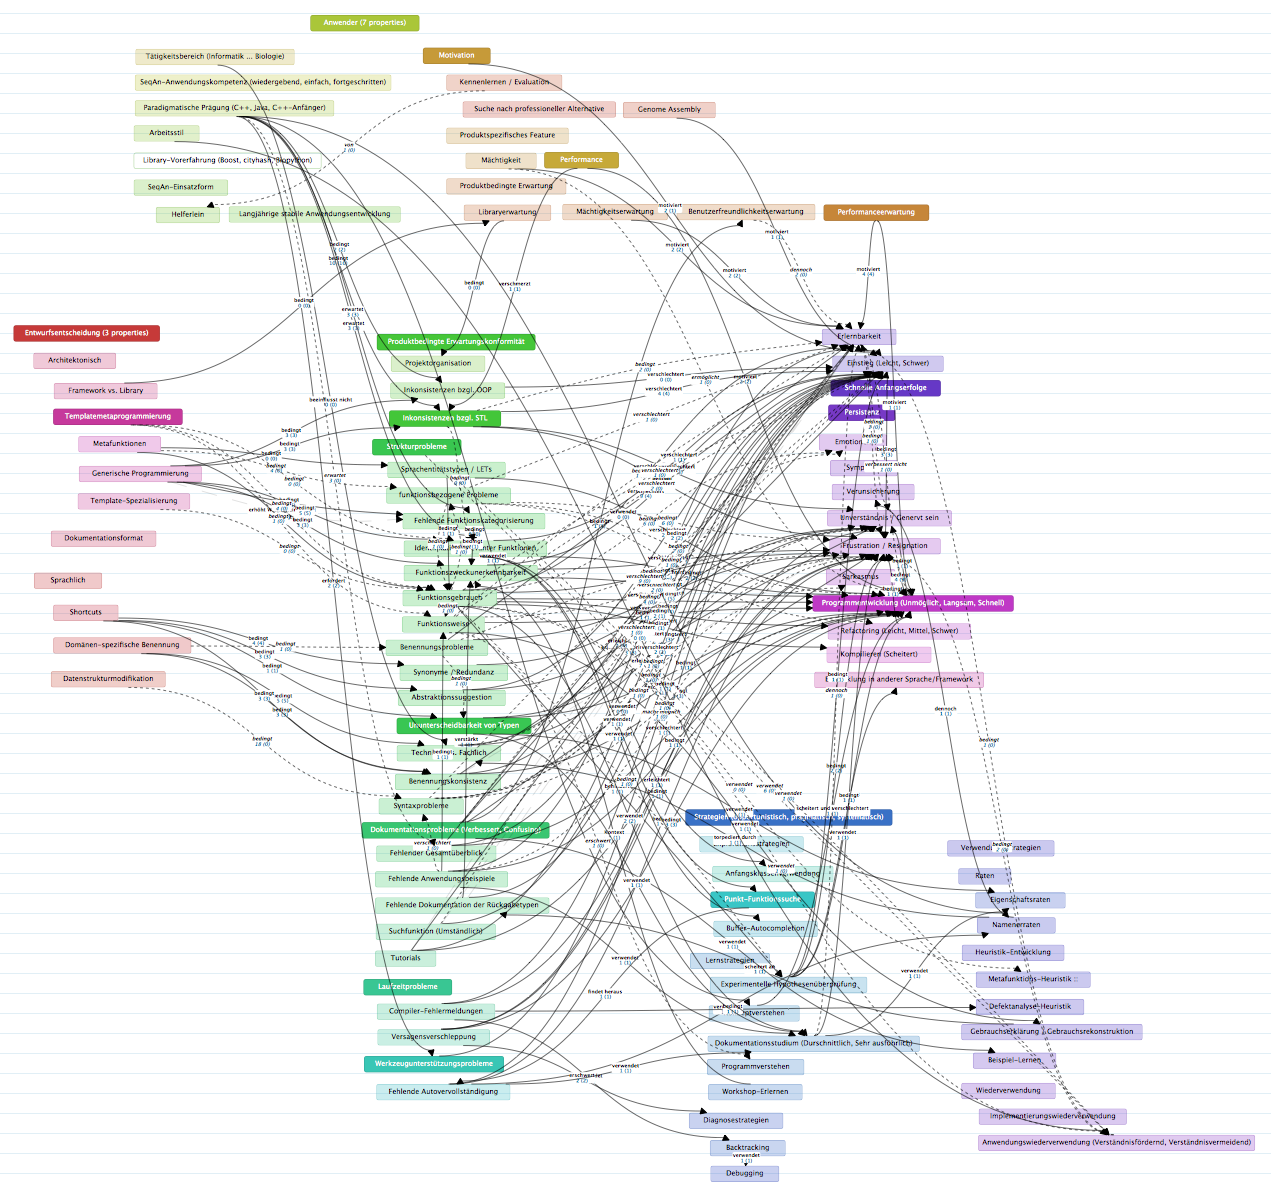
\includegraphics[width=\linewidth]{Figures/research/gt1.png}
                  \caption{Stand: 15.02.2015}
                \label{fig:research-gt1}
        \end{subfigure}%
        \hfill%
        \begin{subfigure}{0.48\linewidth}%
                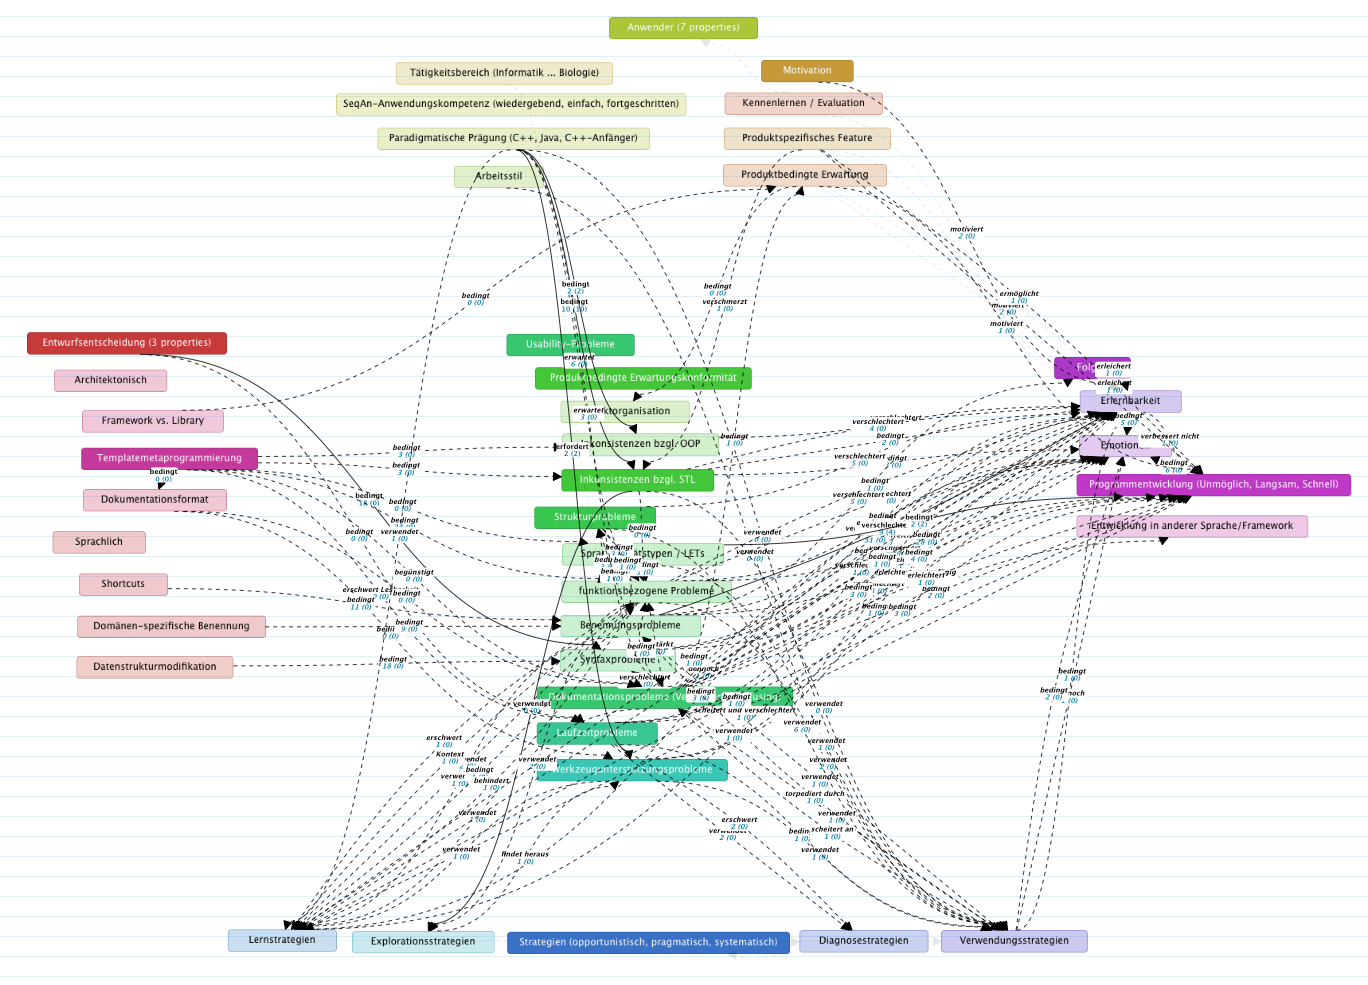
\includegraphics[width=\linewidth]{Figures/research/gt2.png}
                \caption{Stand: 24.03.2015}
                \label{fig:research-gt2}
        \end{subfigure}%
        \caption{Selektives Kodieren in APIUA}%
\end{figure}


\begin{figure}
        \centering
        \begin{subfigure}{0.43\linewidth}
                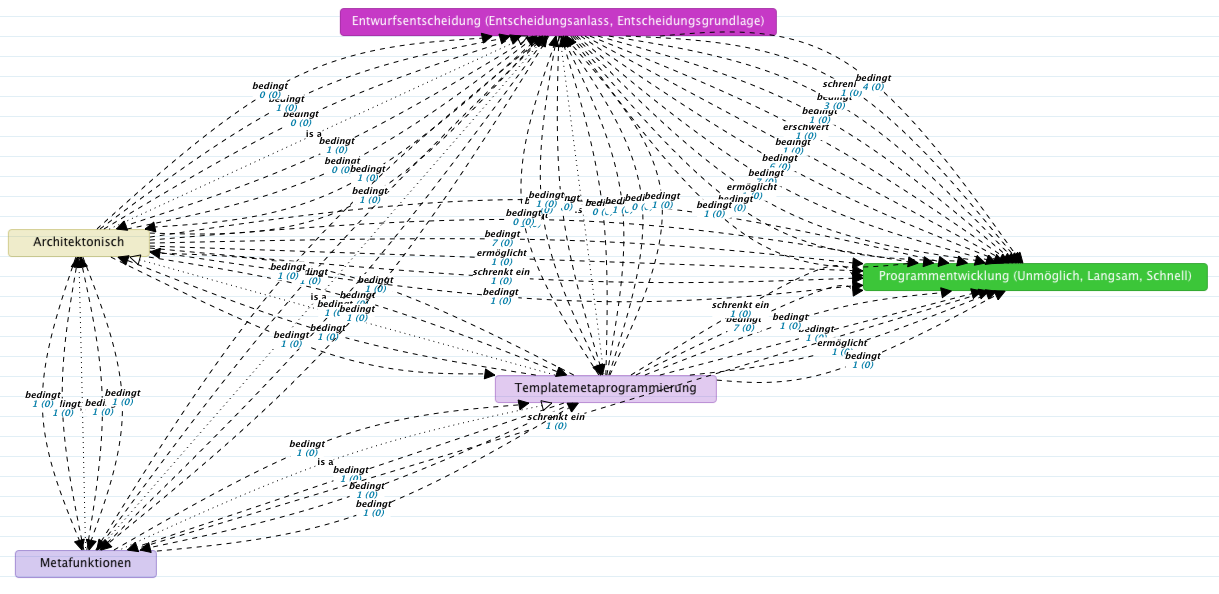
\includegraphics[width=\linewidth]{Figures/research/workflow-selectivecoding-a.png}
                  \caption{ohne Zusammenfassung von hypothetischen Relationen}
                \label{fig:research-workflow-selectivecoding-a}
        \end{subfigure}%
        \hfill%
        \begin{subfigure}{0.43\linewidth}%
                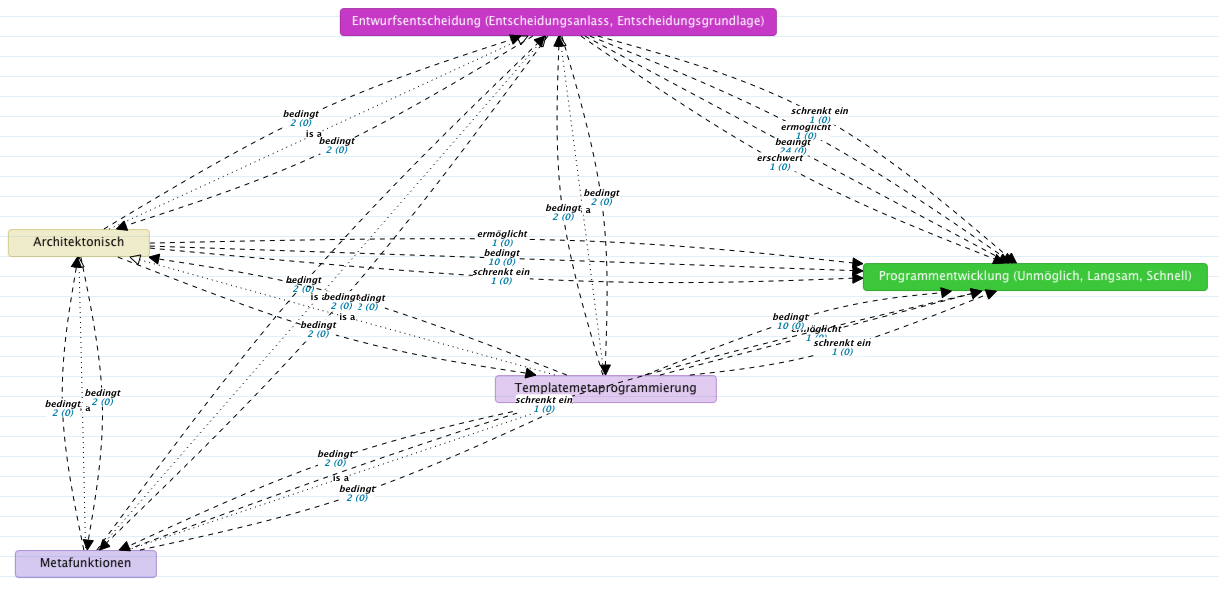
\includegraphics[width=\linewidth]{Figures/research/workflow-selectivecoding-b.png}
                \caption{mit Zusammenfassung von hypothetischen Relationen}
                \label{fig:research-workflow-selectivecoding-b}
        \end{subfigure}%
        \hfill%
        \begin{subfigure}{0.48\linewidth}%
                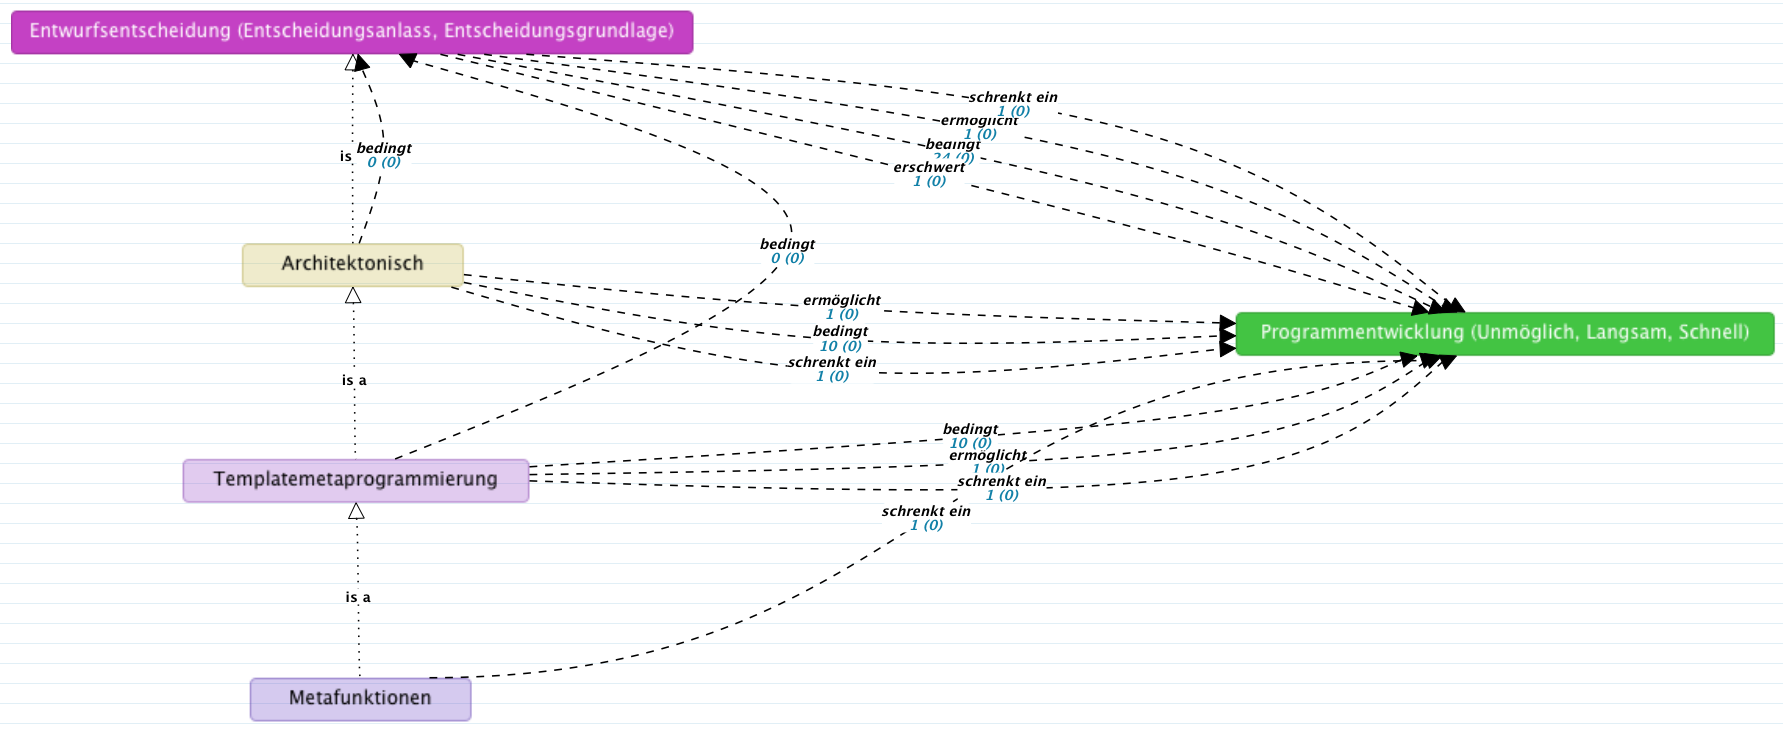
\includegraphics[width=\linewidth]{Figures/research/workflow-selectivecoding-c.png}
                \caption{nach dem Verschieben von zwei Konzepten}
                \label{fig:research-workflow-selectivecoding-c}
        \end{subfigure}%
        \caption{Selektives Kodieren in APIUA mit Hilfe zusammengefasster hypothetischer Relationen}%
        \label{fig:research-workflow-selectivecoding}
\end{figure}




\subsection{Probleme}

Neben den bereits genannten Problemen traten auch solche auf, die den Gebrauch der \gls{gtm} selbst betreffen. Drei Problemklassen stelle ich im Folgenden vor.


\subsubsection{Komplexität und Fokus}
\label{sec:schwierigkeiten-breite}

Empirische Forschungsmethode, zu denen die \gls{gtm} gehört, werden von \cite{SIGCHI:2009up} nur zu Evaluation eines einzelnen API-Aspektes als geeignet betrachtet. Das bestätigen auch andere Studien \citep[vgl. u.a.][]{Stylos:2008jt,Beaton:2008jn,Beaton:2008ix,Ellis:2007kv,Stylos:2007jb}. Ich habe versucht, SeqAn in seiner ganzen Breite zu betrachten, was eine Reihe von Aspekten --- angefangen bei der \code[apiua://code/-9223372036854774893]{Anwenderschaft} bis hin zu \code[apiua://code/-9223372036854775448]{Benennungsproblemen} --- umfasst. Meinen Anspruch, diese Breite in der gegebenen Zeit auch in der selben Tiefe zu betrachten, ist mir nicht vollständig gelungen, wie die Forschungsergebnisse zeigen werden. Darum hatte ich mich entschlossen, mich auf die \code{apiua://code/-9223372036854775515} und die Folgen der \code{apiua://code/-9223372036854775494}{paradigmatischen Prägung} zu konzentrieren, was sich beispielsweise in der geringen Entdeckung von Eigenschaften anderer Konzepte äußert.


\subsubsection{Modellierung der Ergebnisse}
\label{sec:gtm-modellierung}

Die Modellierung meiner Theorie fiel mir alles andere als leicht. Durch die \gls{apiua}-Unterstützung hierarchischer Konzepte stellte sich häufig die Frage, welches Kriterium als Zerlegungskriterium für Unterkonzepte verwendet werden soll und welche Kriterien als Eigenschaften dienen. Für meine Daten haben sich gleich fünf mögliche Konzepte gebildet, die als Elternkonzepte bzw. Zerlegungskriterium für die möglichen Unterkonzepte dienen konnten:

\begin{itemize}
  \item \code{Erwartungskonformität}\\Inwiefern kann existierendes Wissen durch den Anwender wiederverwendet werden?
  \item \code{apiua://code/-9223372036854774950}\\Welche kognitiven Dimensionen sind betroffen?
  \item \code{SeqAn-Feature}\\Mit welcher Funktionalität/Merkmal von SeqAn hat meine Beobachtung zu tun?
  \item \code{apiua://code/-9223372036854775281}\\Welche Art von Entwurfsentscheidung liegt vor?
  \item \code{apiua://code/-9223372036854774939}\\Was für eine Art Usability-Problem liegt vor?
\end{itemize}

Ich glaube, dass dieses Problem nicht nur mit meiner Unerfahrenheit im Gebrauch der \gls{gtm} und der Möglichkeit, Konzepte hierarchisch anzuordnen zu tun hat, sondern auch mit der geringen anwendungsbezogenen Strukturierung der GTM-Literatur \citep[insb.][]{strauss1990basics,strauss1987qualitative,glaser1978theoretical}. In der Dissertation von \cite{Salinger:2013vd} beschreibt der Autor ähnliche Probleme (S. 107 f.) und formuliert vier Praktiken, die ihm dabei halfen diese Probleme zu lösen (S. 108 ff.). Praktik 1 ``Blickwinkel auf die Daten'' hätte mein Modellierungsproblem sicherlich geschmälert, indem mir bewusster gewesen wäre, dass sich mein Blickwinkel auf die Daten ändert und welchen ich gerade habe.

Inhaltlich gesehen gibt es leider keine umfassenden API-Usability-Taxonomien \citep{Daughtry:2009be}, die meine Modellierung vereinfacht haben könnten. Allerdings konnte ich für das oben bereits genannte Konzept \code{apiua://code/-9223372036854775281} auf eine entsprechende Taxonomie von \cite{Stylos:2007ip} zurückgreifen. Taxonomien für Usability-Probleme werden von \cite{Khajouei:2011bm,Keenan:1999di} vorgeschlagen. Beide Taxonomien wurden empirisch, allerdings ausschließlich durch die Auswertung grafischer Benutzeroberflächen mit textuellen Komponenten entwickelt. Einzig \cite{Grill:2012jm} haben sich speziell mit API-Usability-Problemen befasst und für deren Unterteilung die vier Kategorien \textit{Dokumentation}, \textit{Laufzeit}, \textit{Struktur} und \textit{Benutzererlebnis} verwendet.

Ein weiteres Problem ist, dass bestimmte Werte für Eigenschaften gemeinsam mit dem Konzept wiederum ein Konzept bilden können. Beispiel: \code{apiua://code/-9223372036854775281} haben die Eigenschaft \code{apiua://code/-9223372036854774839}, welche die Ordinalskala \textit{(implizit, explizit-intuitiv, explizit-argumentativ, explizit-empirisch)} verwendet. Implizite und explizite-intuitive Entwurfsentscheidungen bilden in meiner Theorie das Konzept \code{Bauchgefühlentscheidung}. Inhaltlich ist das nachvollziehbar und kanonisch. Jedoch ist die technische Realisierung schwierig und führt zu einer weiteren Abstraktionsebene innerhalb einer \acrfull{gt}, weshalb ich diese Funktion nicht implementiert habe.

\label{sec:Datenanalyse-STL-Inkonsistenzen-vereinfachen}
Axiale Kodiermodelle können sehr groß werden, wie die \fref{fig:research-gc-acm} veranschaulicht. Solche Modellierungen auf das Wesentliche zu reduzieren, stellte mich vor große Probleme. Bei deren Reduktion halfen mir das APIUA-Werkzeug durch die Darstellung impliziter und hypothetischer Relationen, auf die ich im \sref{sec:Erkenntnisperspektive} auf Seite \pageref{sec:Erkenntnisperspektive} eingegangen bin.

\begin{figure}
\begin{minipage}{\textwidth}
  \centering
    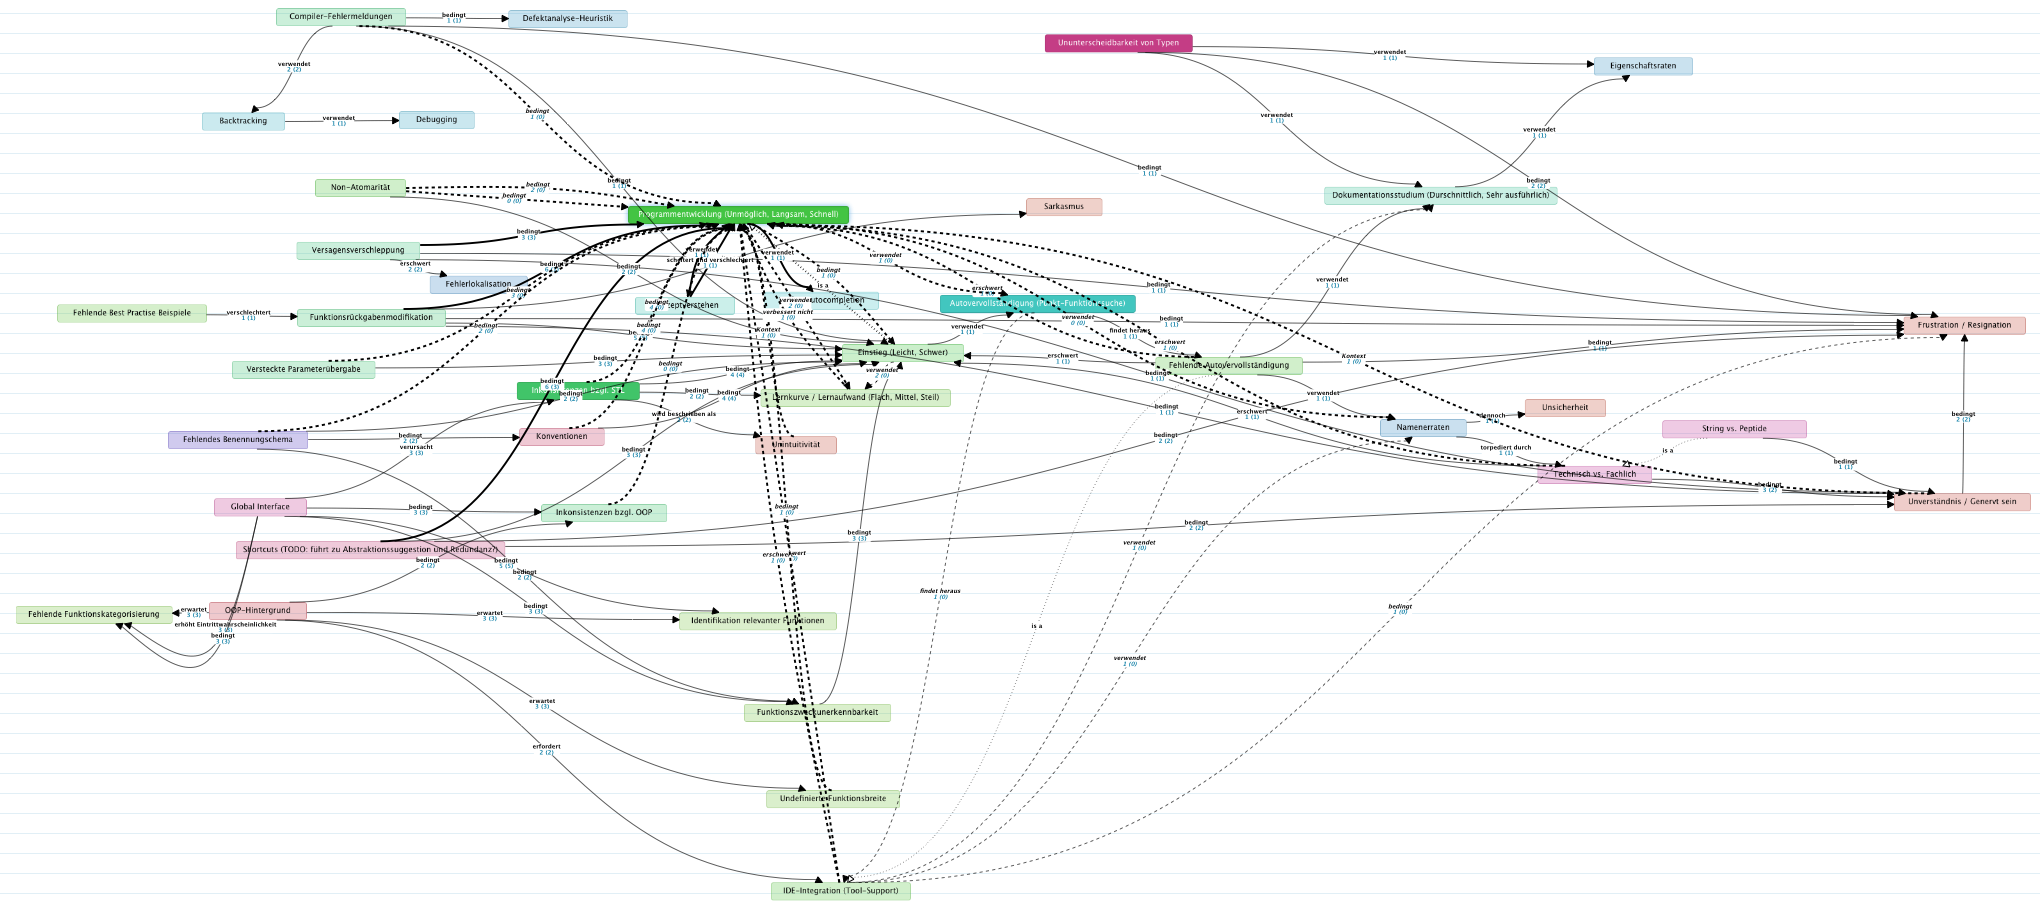
\includegraphics[width=1.0\linewidth]{Figures/research/gc-acm.png}
  \caption[Axiales Kodiermodell zur Gruppendiskussion]{Axiales Kodiermodell zur Gruppendiskussion\citepurl{apiua://axialcodingmodel/0z5ANneuBKhFKJkb}}
  \label{fig:research-gc-acm}
\end{minipage}
\end{figure}




\subsubsection{Validität}
\label{sec:probleme-validierung}

Während die Programmierfortschritte-Daten in situ sind, handelt es sich bei den Cognitive-Dimensions-Fragebögen um Ex-post-facto-Daten, die eine andere Perspektive für die axiale Kodierung im Sinne des paradigmatischen Modells erfordern. Darüber musste ich mir erst durch mehrere Analyseanläufe bewusst werden. Das betrifft insbesondere das axiale Kodieren von mehr als einem Fragebogen: Lässt sich beispielsweise in einem Fragebogen die Relation \rel[]{\code{apiua://code/-9223372036854774928}}{\code{apiua://code/-9223372036854774927}} und in einem anderem Fragebogen die Relation \rel[]{\code{apiua://code/-9223372036854774927}}{\code{apiua://code/-9223372036854774926}} finden, kann daraus nicht ohne Weiteres auf einen Zusammenhang \rel[]{\code{apiua://code/-9223372036854774928}}{\code{apiua://code/-9223372036854774926}} geschlossen werden. Dazu würde ein gutes Verständnis vom Kontext vorliegen müssen, der den Fragebögen häufig aber kaum zu entnehmen ist.

Im Gegensatz zu den Programmierfortschritte-Daten, sind die subjektiven Datenquellen häufig ärmer an Kontextinformationen. Beide Datenquellen waren aber überraschend breit in ihrem Aussagegehalt, was dazu führte, dass ich viele Konzepte entdecken, aber nur wenige Verankerungen/Phänomene dazu finden konnte.
% Aus Zeitgründen, konnte ich nicht jedes Konzept in den Programmierfortschritte-Daten suchen und damit triangulieren
Dies führte mich zu der Frage, welche Aussagekraft überhaupt die Anzahl der zu einem Konzept gefundenen Phänomene haben. In einer \gls{gtm} der zweiten Generation \citep{charmaz2006constructing} können textuelle Daten explizit Wort-, Zeilen- und Absatz-weise kodiert werden, was massiven Einfluss auf die Anzahl gefundener Phänomene hat. Entsprechend eignet sich dieses quantitative Maß nur bedingt nur Diskussion der Validität.




\begin{comment}

\subsection{Anekdoten}
%TODO schreiben am Ende
In diesem letzten Abschnitt möchte ich an Hand konkreter Beispiele darstellen, wie ich die \gls{gtm} angewendet und inwieweit sie mir beim Erkenntnisgewinn und der Generierung einer validen \gls{gt} geholfen hat.


\subsubsection{Vorteile qualitativen Forschung}
- 3 Phänomene mit Code "Mächtigkeit" kodiert
- Phänomene waren Antworten auf die Frage nach der Work-Step Unit von SeqAn
- Erkenntnis: SeqAn bekommt durch die 3 Teilnehmer eine gute WSU bescheinigt bekommen
- schließlich war der Fragebogen mit großer Sorgfalt und basierend auf dem von Green und Clarke (Ausrichtung nach API) entworfen worden
- ABER: stimmt die Erkenntnis?
- Die 3 befragten waren Teilnehmer der Workshops
- Alle hatten mit SeqAn nur Kontakt innerhalb des Workshops und dabei vornehmlich Tutorials bearbeitet
- Folge: Sie konnten die Frage nicht adäquat beantworten. Stattdessen haben Sie (unbewusst) Äußerungen zu dem gemacht, was sie sich von SeqAn versprechen (aus irgendeinem grund müssen sie ja beim Workshop sein)
- Der Code heißt nun Mächtigkeitseindruck apiua://code/-9223372036854775568
- abstraktives Fazit: Das die Anwendungsdauer auf die Interpretation der anderen Antworten Auswirkungen hat, kann man nur qualitativ herausfinden


\subsubsection{Paraphrasierung und wortgenaue Analyse}
Wortgenaue Analyse: \citep{charmaz2006constructing}
Annekdote Paraphrasierung und wortgenaue Analyse (gelernt im Seminar)
- ~hilft den Kern einer Aussage zu erfassen
- kann aber auch helfen, eine Aussage erst auswerten zu können (aufgrund der fehlenden Klammerung in der Sprache zum Beispiel)

- Aussage apiua://survey/cd/2013-09-19T11:51:16.616+02:00/hardMentalOperations:
Yes, remembering all the templates and variants of types and templates and trying to figure out what is the difference between say Dna5 and Dna5String.

Remembering bezieht sich klar auf templates und variants. Aber bezieht sich variants auch auf type and templates oder nur auf type und "and templates" ist ein dritter Aufzählungspunkt (Sprache ist nicht immer perfekt).
Also:

Stichpunktartige Paraphrase:
- remembering complicated
-- many templates
-- many variants of types
-- many variants of templates
- difference unclear
-- e.g. Dna5 and Dna5String

Kodierung
> Fachliche Inkorrektheit, apiua://code/-9223372036854775335
"many variants of types', 'Dna5 and Dna5String"

> Metafunktionen, apiua://code/-9223372036854775514
'many templates", Das Konzept Metafunktion selbst is neu/umfangreich.

> Typing, apiua://code/-9223372036854775352
'many variants of types and templates"
~ umfasst nämlich Metafunctionsaufrund die Angabe von Typen



Sehr gutes Beispiel in apiua://survey/cd/2013-09-19T11:51:16.616+02:00/hardMentalOperations



\subsubsection{Ständiges Vergleichen}
- ACM verwendet, um fehlende Relation zu finden.
Beispiel Group Discussion ACM
Bild: missing\_relations.png
Code Konventionen hatte keine ausgehende Relation 
Alle Citations geprüft und mit "erschwert Einstieg" nachkodiert



\subsubsection{Annekdote für Kompetezaufbau / theoretische Sensibilität / zu klären}
- Antwort auf die Frage nach der Viscocity von SeqAn (apiua://survey/cd/2013-09-18T17:50:13.425+02:00/viscosity)
"Wenn es wenig Beispiele gibt bzw. die Funktionalitaet mancher Konstrukte zu ergruenden ist"
- unklare Aussage
- Progressive Evaluation-Frage an anderen Teilnehmer apiua://survey/cd/2013-09-18T17:50:13.425+02:00/progressiveEvaluation: "Wenn man lange nach bestimmten Funktionen sucht bzw. lange braucht deren Verwendung zu verstehen ist der Fortschritt manchmal schwer zu ueberblicken."
- Hier wurde klar, was der andere mit "Funktionalitaet" meinte: Nämlich "Funktionsweise"


\subsubsection{Vereinfachung}
Annekdote für Minimalismus-Drang:
- Frage nach Cd-Work Step Unit
- Sehr viel. Aber ich denke wenig Code ist auch nicht immer die beste Lösung.
Bei seqAn finde ich es etwas zu wenig, da ich als Anfänger die Schritte nicht sehe die in einer Zeile stecken und es mir dadurch schwer fällt nachzuvollziehen was hier genau passiert.
- Ursprünglich kodiert als "Nachvollziehbarkeit".
- Später nochmal gesamten Fragebogen gelesen. User beklagt sich über technische Verständnisschwierigkeiten in anderen Fragen (z.B. keine Dokumentation der Rückgabetypen.
- Überlegung, ob nicht doch nur C++-Sprachkenntnisse fehlen
- ABER: In Frage nach Premature Commitment wird Generizität globaler Funktionen gelobt $\rightarrow$ also doch Kenntnisse
- Die Work-Step-Unit ist tatsächlich zu groß.Der Code bleibt "Nachvollziehbarkeit" oder so ähnlich (apiua://survey/cd/2013-09-18T17:45:54.889+02:00/workStepUnit)



\subsubsection{Verständnisschwierigkeiten (schlechtes Englisch)}
Aussage von apiua://survey/cd/2013-09-18T17:50:37.900+02:00/hardMentalOperations
Verschiedene Lesarten für "I feel that you need to get use to available functions to make things work.":
1. Ich muss mich erst an die vorhandene Funktionalität gewöhnen.
2. Ich muss erst verstehen, welchen Funktionen überhaupt bereit stehen.

Entscheidung in Anbetracht seines in den anderen Fragen geäußerten Kenntnissstandes (bloody beginner): 1



\subsubsection{Voreingenommenheit}
- Aussage zur Work-Step Unit Frage: apiua://survey/cd/2013-09-18T17:45:54.889+02:00/workStepUnit: 
- Kodierung: "Verständnis Funktionsweise" mit Wert "Abstrahiert", Memo: "Abstrahiert: Der Grad der Abstraktion verbirgt die einzelnen Ausführungsschritte, was das Verständnis erschwert.
Möglich Ursache: Zu große Work-Step Unit"
- Erst mit der Aussage apiua://survey/cd/2013-09-18T17:45:54.889+02:00/roleExpressiveness wurde klar, dass in beiden Fällen die Strategie beschrieben wird, wird der Befragte mit fehlenden (oder unzureichenden / unpassenden) Anwendungsbeispielen umgeht. Er erklärt sich die Anwendung dann mit dem Funktionsablauf und der Rückgabe. siehe apiua://code/-9223372036854775401, mit Work-Step Unit hat das herzlich wenig zu tun oder höchstens insoweit, als dass sie das Problem hier abgeschwächt hätte


\subsubsection{Soziale Erwünschheit und Vorbelastung}
apiua://survey/cd/2013-09-18T17:46:55.042+02:00/learningStyle sagt die Tutorials seien hilfreich; sagt aber auch "zum größten Teil" und schränkt im folgenden Satz weiter ein.
Die Tutorials wurden von mir überarbeitet. Erst der Blick durch eine zweite Person brachte diese neue Perspektive.



\subsubsection{Theoretisches Sampling}
- zeigt, wie Reichhaltig die Daten sind und sind ein Qualitätsmerkmal für meine Art der Datenerhebung
Annektode Existierende Quellen nochmals sichten:
Manchmal und gerade am Anfang sieht man bestimmte Aspekte einer Aussage nicht. Man ist für sie blind. Erst wenn man die notwendige Sensibilität und/oder einem dieser Aspekt auf dem Silbertablett präsentiert wird, muss man in sein bereits kodiertes Material zurückkehren und Phänomene für diesen Aspekt suchen.
Geschehen bei apiua://code/-9223372036854775314 - Frustation. Aufmerksam geworden bei "99\% of the cases when I refactor something first version will not even compile." apiua://survey/cd/2013-09-19T11:51:16.616+02:00/viscosity und dann auch Dinge wie "Meistens lassen sich Dinge nicht überprüfen, weil der Code nicht kompiliert. Das Prototypen von Dingen fällt mir oft sehr schwer." apiua://survey/cd/2013-09-18T17:46:55.042+02:00/progressiveEvaluation dessen Frustration man sehr gut im Kontext seiner anderen Antworten (wiederholt "schwer", "sehr schwer", "nicht leicht") sehen kann 


\subsubsection{Reliabilität}
- ein drei Wochen alte Quelle apiua://survey/cd/2013-09-19T11:51:16.616+02:00/workStepUnit ein drittes Mal kodiert (ohne auf alte Codes zu schauen)
- erst: Glaube, als gefunden Codes bereits gefunden zu haben.
- dann: ein neuer Code; noch einmal überlegt. Nein, dieser neue Code ''Overhead`` ist nur ein Aspekt von Work-Step Unit (TP erfordert die Berechnung von Typen und macht damit Ausdrücke syntaktisch komplexer - länger als ohne)
- Vergessene Codierschritte exakt identisch gemacht, sogar gleiche Zitate rausschreiben wollen
=> gutes Zeichen



\subsubsection{Refactoring}
-apiua://survey/cd/2013-09-18T17:45:54.889+02:00/hardMentalOperations
"Hard Mental Operations: Eingentlich nicht. Es braucht sicher etwas Übung. Aber dafür sind die guten Assignments sehr Hilfreich."
Bisher kodiert als "Lernfortschritt mittels Assignment"
Dann wurde aber klar, dass es sich um zwei Formen handelt:
1. Die Bearbeitung der Assignments im Rahmen der Bearbeitung von Tutorials (TODO: Code nennen)
2. Eine Strategie, die eingesetzt wird, sobald die Programmentwicklung ins Stocken gerät (TODO: Code nennen)

\end{comment}











%Allgemein:
%Exakte GT - insbesondere mit der Modellierung von Eigenschaften - bei der Fülle an Bedienungsproblemen äußerst komplex. Man müsste entweder erheblich mehr Zeit investieren, oder die Betrachtungsbreite einschränken.
%Daher Clustering-Ansatz gewählt, bei dem Codes gruppiert sind (und damit implizit Eigenschaften enthält).
%Beispiel:
%Professionelle Programmentwicklung, Einstieg, Herumprobieren könnten alle der Code Programmentwicklung mit den Eigenschaften Zweck/Ziel (Produktion, Erlernen) und Temporalität (Persistent, Temporär) sein. Professionelle Programmentwicklung wäre dann Produktion+Persistent, Einstieg (Erlernen+Persistent) und Herumprobieren (Erlernen, Temporär)

%Vereinfachtes axiales Kodieren:
%Paradigmatisches Modell, das wie eine visuelle Schablone (TODO Grafik) gelesen werden soll.
%Umdefinition von Kontext: Alle Konzepte, die das interpretatorische Bild vervollständigen (Hintergrundinformationen,
%die Einfluss haben können) (also nicht: Eigenschaften-Auswahl von XXX und Ursache)
%Umdefinition von XXX: Alle Konzepte, die belegt Einfluss auf zentrales Phänomen haben. 



\subsection{Zusammenfassung}

In dieser Phase 4 habe die eigentliche Forschung mit Hilfe der \gls{gtm} und meinem Datenanalysewerkzeug \gls{apiua} besprochen. Dazu habe ich zunächst die Forschungsmethoden anderer Studien vorgestellt. Dabei bin ich auf die Eignung und die seltene Verwendung der \gls{gtm} für explorative Studien eingegangen. Ich habe den unterschiedlichen Gebrauch der \gls{he} erläutert und bin auf die Schwächen anderer Forschungsmethoden eingegangen.

Anschließend habe ich die Analyse der Programmierfortschritte-Daten, der Cognitive-Dimensions-Fragebögen und der Gruppendiskussion beispielhaft skizziert und die konkrete Umsetzung innerhalb von \gls{apiua} dargestellt.

In meiner Beschreibung des selektiven Kodierens, habe ich erläutert, welchen Beitrag die Konzepte \code{apiua://code/-9223372036854775633} und \code{apiua://code/-9223372036854775494} beim Durchbruch meiner Forschung hatten und welche APIUA-Funktionen mir bei der Reduktion des ``globalen'' axialen Kodiermodells auf ein theoretisches Kodiermodell behilflich waren.

Weiterhin bin ich auf Komplexitäts-, Modellierungs- und Validitätsprobleme beim Gebrauch der \gls{gtm} eingegangen.% und habe meine Forschungsgenauigkeit anekdotisch beschrieben.